%%%%%%%%%%%%%%%%%%%%%%%%%%%%%%%%%%%%%%%%%%%%%%
%%%%%%%%%%%%%%%%%%%%%%%%%%%%%%%%%%%%%%%%%%%%%%
\documentclass[12pt,a4paper,portuges]{article}
\usepackage{relat_siger}
\usepackage{epstopdf}
%%%%%%%%%%%%%%%%%%%%%%%%%%%%%%%%%%%%%%%%%%%%%%
%inclusao do arquivo de macros
\input macros.tex
\newcommand{\perm}{\kappa}
\newcommand{\ver}{$\mathbb{VER}$ }
\newcommand{\vaz}{Q}
\newcommand{\hd}{h}
%\newcommand{\fig}{Fig.~}
\newcommand{\cpy}{\xi}
\newcommand{\LU}{{LU}}
\newcommand{\m}{$M$}
\newcommand{\mm}{M}
\newcommand{\xx}{x_{1}}
\newcommand{\y}{x_{2}}
%\renewcommand{\cov}{\mathcal{C}}
%\renewcommand{\covv}{\cov(\xx,\cpy)}
\newcommand{\kl}{KL}
\newcommand{\KL}{{Karhunen-Lo\`eve}}
\newcommand{\Y}{{Y}}
\newcommand{\Ym}{\hat{Y}}
%\newcommand{\vw}{\ale}
\newcommand{\ale}{\omega}
\newcommand{\Dom}{\mathcal{D}}
\newcommand{\Yxw}{\Y(\vx,\ale)}
\newcommand{\ava}{\lambda}
\newcommand{\avai}{\ava_{i}}
\newcommand{\avaj}{\ava_{j}}
\newcommand{\ave}{\phi}
\newcommand{\avei}{\ave_{i}}
\newcommand{\avej}{\ave_{j}}
\renewcommand{\exp}{\mbox{exp}}
\newcommand{\normal}[2]{\mathbb{N}(#1,#2)}
\newcommand{\clen}{\ell} % correlation length
\newcommand{\D}{\mathcal{D}}
\newcommand{\mcmc}{\textsf{McMC}} % Monte Carlo method
\newcommand{\apri}{{\em a priori}}
\newcommand{\apost}{{\em a posteriori}}
%%%%%%%%%% alteracoes marcio %%%%%%%%%%%%%%%%%
\newtheorem{coment}{Análise}[subsection]
%%%%%%%%%%%%%%%%%%%%%%%%%%%%%%%%%%%%%%%%%%%%%%
\hyphenation{}
%define o numero de secoes
\setcounter{secnumdepth}{3}
%define o numero de secoes no sumario
\setcounter{tocdepth}{3}
%\includeonly{}
\makeindex
\begin{document}
\AddToShipoutPicture*{\BackgroundPic}
\begin{titlepage}
%
%
\hspace{-26.5mm}
\noindent \begin{minipage}[t][1.5cm][l]{2.2cm} 
\scriptsize
\centering
\raisebox{1pt}{\includegraphics[height=40pt]{/prj/prjmurad/mrborges/Dropbox/latex/figuras/lnccbf.eps}}
\makebox[\textwidth][s]{{\sf\textbf{L}\ \ a b o r a t ó r i o}}\par\vspace{-0mm}
\makebox[\textwidth][s]{{\sf\textbf{N} a c i o n a l \ de}}\par\vspace{-0mm} 
\makebox[\textwidth][s]{{\sf\textbf{C} o m p u t a ç ã o}}\par\vspace{-0mm}
\makebox[\textwidth][s]{{\sf\textbf{C} i e n t í f i c a}}\par
\end{minipage}
%
\vspace{-20mm}
\begin{center}
 \hspace{10mm}
\raisebox{1pt}{\includegraphics[height=70pt]{/prj/prjmurad/mrborges/Dropbox/latex/figuras/SIGER_logo.eps}}
\end{center}
%
\begin{center}
{\vspace{10mm}\textbf{\Large \sf }\\
\vspace{50mm}
\hspace{20mm}\textbf{\Huge \sf Geração Numérica de}\\
\hspace{20mm}\textbf{\Huge \sf Campos Aleatórios}}
\end{center}
%
\begin{flushright}
\vspace{30mm}
  \textbf{Autor:} Marcio Borges
\vspace{50mm}
\end{flushright}
%
	\begin{center}
	{Petrópolis-RJ\\ \today }
	\end{center}
%
\clearpage
%\pagestyle{empty}
\small
\pagenumbering{roman}
\tableofcontents
%\clearpage
%\listoffigures
%\clearpage
%\listoftables
\end{titlepage}
\setcounter{page}{1}
\pagenumbering{arabic}
%%%%%%%%%%%%%%%%%%%%%%%%%%%%%%%%%%%%%%%%%%%%%%%%%%%%%%%%%%%%%%%%%%%%%%%%%%%
%%%%%%%%%%%%%%%%%%%%%%%%%%%%%%%%%%%%%%%%%%%%%%%%%%%%%%%%%%%%%%%%%%%%%%%%%%%
%\onehalfspacing
\section{Geração Numérica de Campos Aleatórios}
O conhecimento sobre a heterogeneidade de um meio poroso normalmente é incompleto devido a escassez
de informações sobre o mesmo, o que nos leva à necessidade de fazermos uma descrição probabilística
de suas propriedades. Neste sentido, as heterogeneidades das propriedades dos reservatórios (por
exemplo, a permeabilidade, a porosidade e o módulo de Young) são representadas por campos
aleatórios, com propriedades estatísticas específicas que serão gerados por três metodologias:
Decomposição LU, Decomposição de Karhunen-Loève e Labtran-Geo. Desta forma, o objetivo deste
relatório é apresentar os geradores construídos para serem utilizados no projeto:
\uppercase{Modelagem e Simulação Numérica de Escoamentos em Reservatórios Heterogêneos com
Acoplamento Geomecânico} dentro da rede SIGER.

%%%%%%%%%%%%%%%%%%%%%%%%%%%%%%%%%%%%%%%%%%%%%%%%%%%%%%%%%%%%%%%%%%%%%%%%%%%
\subsection{Campos}
Neste trabalho, serão gerados somente campos em domínios retangulares com malhas também
retangulares.
Para padronizar tanto a geração quanto a utilização destes campos nos simuladores desenvolvidos
apresentamos, a seguir, a formatação dos campos. Tomaremos como exemplo a representação esquemática
de um campo aleatório posto em um domínio retangular $\Omega$ com dimensões físicas $L_{1}\times
L_{2}$, discretizado em uma malha de $n_1\times n_2$ elementos ($10\times 5$ neste exemplo),
conforme apresentado na \fig{omega}.
\begin{figure}[H]
\centering
  \input{figuras/malha.pstex_t}
  \caption{Representação esquemática de um campo aleatório posto em um domínio bidimensional
$\Omega$.}
\label{omega}
\end{figure}

%%%%%%%%%%%%%%%%%%%%%%%%%%%%%%%%%%%%%%%%%%%%%%%%%%%%%%%%%%%%%%%%%%%%%%%%%%%
\subsubsection{Formato dos arquivos de dados}

Nos geradores desenvolvidos neste projeto os arquivos de saída, com extensão {\em *.dat}, possuem o
seguinte formato:

\clearpage

\begin{flushleft}
\footnotesize
\begin{verbatim}
1.000000
0.400000
10
5
1
0.500000
2
2
0
0.909149 -0.661580 -0.397227 0.308463 0.180042 
0.015598 -0.849240 -0.458387 0.201703 0.100701 
192837465
1
0.110745 -0.825363 0.365615 0.268071 ...
\end{verbatim}
\end{flushleft}

\noindent que, de acordo com a \fig{omega}, as quatro primeiras linhas trazem informações sobre as
dimensões físicas de $\Omega$, sendo que a primeira representa o valor de $L_1$, a segunda $L_2$, a
terceira $n_1$, e a quarta $n_2$. Estes dois últimos valores são os números de blocos na direção
$x_1$ e $x_2$, respectivamente. Os dois valores seguintes (quinta e sexta linhas) trazem informações
sobre a covariância do campo. O quinto valor indica que o campo é exponencial se for igual a $1$ e
fractal caso seja $2$. O valor da sexta linha é o do coeficiente de correlação $\lambda$ se o campo
é exponencial ou o expoente de Hurst $\beta$, se o campo é fractal. Os dois valores seguintes
(sétima e oitava linha) não possuem utilidade.

Após as oito primeiras linhas, estão as indicações sobre o valor e a posição de cada bloco. O número
zero indica a primeira linha ($l_0$). Para este caso específico os dez números seguintes são os
valores do campo nos blocos de 1 a 10, respectivamente. O número ${192837465}$ é uma ``bandeira''
que indica o final de uma linha. 

%%%%%%%%%%%%%%%%%%%%%%%%%%%%%%%%%%%%%%%%%%%%%%%%%%%%%%%%%%%%%%%%%%%%%%%%%%%%%%%%
%%%%%%%%%%%%%%%%%%%%%%%%%%%%%%%%%%%%%%%%%%%%%%%%%%%%%%%%%%%%%%%%%%%%%%%%%%%
\subsubsection{Descrição dos campos}\label{descriccao_xi}

Neste projeto consideraremos campos de permeabilidades aleatórios, 
escalares, com distribuição log-normal:
\begin{equation}
	\cond(\vetor{x}) = \cond_{0}e^{\varrho {Y}(\vetor{x})},
\label{campok}
\end{equation}

\noindent onde $\cond_{0}, \ \varrho \in \mathbb{R}$ e  ${Y}(\vetor{x})$ é  um
campo gaussiano aleatório, estacionário, caracterizado por sua  média $\langle
{Y}(\vetor{x})\rangle = 0$ e sua função de covariância  
\begin{equation}
	\mathcal{C}(\vetor{x}, \vetor{y}) = \langle {Y}(\vetor{x}){Y}(\vetor{y})
\rangle,
\label{cov}
\end{equation}

\noindent 
 Na notação acima $\langle \cdot \rangle$ denota a média amostral
(esperança) e $\sigma$ o desvio padrão 
da variável $Y$. 


A  média $\langle \cond(\vetor{x}) \rangle$ e o desvio padrão $\sigma_{\cond}$ do campo
$\cond(\vetor{x})$ são determinados pelos coeficientes $\cond_{0}$ e $\varrho$, respectivamente.
Mudanças no valor de $\varrho$ alteram o coeficiente de variação,
\begin{equation}
	CV_{\cond} \equiv \frac{\sigma_{\cond}}{\langle \cond(\vetor{x})
\rangle},
\label{cv}
\end{equation}

\noindent do campo correlacionado. O coeficiente de variação é utilizado como uma medida
adimensional da heterogeneidade do campo de permeabilidades. 

%%%%%%%%%%%%%%%%%%%%%%%%%%%%%%%%%%%%%%%%%%%%%%%%%%%%%%%%%%%%%%%%%%%%%%%%%%%%%%%%%%%%
\subsubsection{Funções de Covariância Adotadas}

Consideramos neste trabalho formações geológicas 
caracterizadas por campos aleatórios com dois tipos de função de
covariância: fractal e exponencial. 

Para modelos em que introduzimos variabilidade sobre todas as
escalas de comprimento,  tal como no caso de formações 
sedimentares \citep{hewett86} usamos campos nos quais a sua função de covariância 
é dada pela lei de potência:
\begin{equation}
	\mathcal{C}(\vetor{x}, \vetor{y}) = |\vetor{x}-\vetor{y}|^{-\beta},
	\quad \beta > 0.
\label{covpot}
\end{equation}

O expoente $\beta$, chamado de coeficiente de Hurst\index{coeficiente de Hurst},
controla a importância relativa dos comprimentos de escala ``grandes'' e
``pequenos'' na geologia. Portanto, maiores valores de $\beta$ enfatizam os
comprimentos de escala ``pequenos''. Por outro lado, para menores valores de
$\beta$ os comprimentos de escala ``grandes'' são enfatizados. No caso em que
$\beta \to \infty$ obtém-se o caso em que as variáveis são independentes.

Nos casos em que somente as pequenas escalas prevalecem consideraremos campos
com função de covariância  exponencial:
\begin{equation}
	\mathcal{C}(\vetor{x}, \vetor{y}) =
\exp{-\frac{|\vetor{x}-\vetor{y}|}{\lambda}}
\label{covpote}
\end{equation}

\noindent onde $\lambda > 0$ é  o comprimento de correlação.

%%%%%%%%%%%%%%%%%%%%%%%%%%%%%%%%%%%%%%%%%%%%%%%%%%%%%%%%%%%%%%%%%%%%%%%%%%%%%%%%
\section{Métodos de Geração de Campos Aleatórios}

Vários métodos têm sido utilizados para gerar campos aleatórios, 
tais como: {\em
Turning Bands Method} \citep{mantoglou82,oh98}, Método de Decomposição \LU\ de Matrizes ({\em Matrix
Composition Method}) \citep{clifton82,elishakoff83}, Adição Sucessiva Aleatória ({\em Successive
Random Addition}) \citep{oh98,kikkinides99,kikkinides00}, Métodos Espectrais ({\em Spectral
Methods}) \citep{bruining97}, Método da Convolução \citep{furtado90,glimm93}, Método da Expansão KL
\citep{karhunen46,loeve55} e o Método LABTRAN-GEO \citep{mrborges08g}. Todos estes métodos
apresentam vantagens e desvantagens tanto do ponto de vista computacional quanto da qualidade
estatística dos campos. Mais especificamente, no presente projeto, implementamos e estudamos os
métodos de Decomposição \LU, da Expansão KL e o LABTRAN-GEO para gerar campos, que serão empregados
nas simulações de Monte Carlo.

%%%%%%%%%%%%%%%%%%%%%%%%%%%%%%%%%%%%%%%%%%%%%%%%%%%%%%%%%%%%%%%%%%%%%%%%%%%
\subsection{Expansão de Karhunen-Loève (\kl)}
\label{chap:mod_estocastica}
%%%%%%%%%%%%%%%%%%%%%%%%%%%%%%%%%%%%%%%%%%%%%%%%%%%%%%%%%%%%%%%%%%%%%%%%%%%
Uma das metodologias escolhidas para a geração de campos aleatórios, neste projeto, é o Método de
\KL\,desenvolvido, de forma independente, por  \cite{karhunen46} e \cite{loeve55} com base na
decomposição da função de covariância em seus auto-pares. Neste método, um campo aleatório pode ser
representado como uma expansão envolvendo um conjunto de funções determinísticas com seus
respectivos coeficientes aleatórios.

%%%%%%%%%%%%%%%%%%%%%%%%%%%%%%%%%%%%%%%%%%%%%%%%%%%%%%%%%%%%%%%%%%%%%%%%%%%
\textbf{Definição:}
%%%%%%%%%%%%%%%%%%%%%%%%%%%%%%%%%%%%%%%%%%%%%%%%%%%%%%%%%%%%%%%%%%%%%%%%%%%
Considere um campo aleatório $\Y(\vx,\ale)$ definido sobre um espaço de probabilidades
$(\Omega,\events,\probab)$ composto pelo espaço amostral, conjunto de eventos e uma medida de
probabilidade, respectivamente, e indexado a um domínio limitado $\Dom$. O campo $\Y$ pode ser
escrito como 
%
\begin{equation}
  \Yxw = \med{\Y(\vx)} +\sum_{i=1}^{\infty}\sqrt{\avai} \avei(\vx)
\xi_{i}(\ale),
\label{kl}
\end{equation}
%
\noindent onde $\avai$ e $\avei$ são os auto-valores e as auto-funções da função de covariância
$\covv{\Y}$, respectivamente. Por definição,  $\covv{\Y}$ é limitada, simétrica e definida positiva
e tem a seguinte auto-decomposição:
%
\begin{equation}
  \covv{\Y} = \sum_{i=1}^{\infty} \avai\avei(\vx)\avei(\vy).
\label{klcov}
\end{equation}
%

Os auto-valores e auto-funções de \eq{klcov} são as soluções da equação integral de Fredholm dada
por
%
\begin{equation}
  \int_{\Dom} \covv{\Y} \avei(\vx) d\vx = \avai\avei(\vy).
\label{fred}
\end{equation}
%
\noindent A solução de \eq{fred} forma um conjunto completo de auto-funções ortogonais,
quadrado-integráveis, que satisfazem a equação
%
\begin{equation}
  \int_{\Dom} \avei(\vx) \avej(\vx)=\delta_{ij},
\end{equation}
%
\noindent na qual $\delta_{ij}$ é a função delta de Kronecker.

O conjunto de variáveis aleatórias não-correlacionadas $\xi_{i}(\ale)$ pode ser expresso como
%
\begin{equation}
  \xi_{i}(\ale) = \displaystyle
\frac{1}{\sqrt{\avai}}\int_{\Dom}\flu{\Y}\avei(\vx) d\vx,
\end{equation}
%
\noindent onde $\flu{\Y}$ é a flutuação.

Se os autovalores $\avai$ decaem rapidamente então podemos truncar a expansão \eq{kl} e utilizar
apenas poucos termos para representar o campo, reduzindo assim a dimensão do espaço de
parâmetros. Portanto, para implementação prática do método, a série é truncada em um número finito
de termos, digamos  \m, obtendo
%
\begin{equation}
  \Ym(\vx,\ale) = \med{\Y(\vx)} +\sum_{i=1}^{\mm}\sqrt{\avai} \avei(\vx)
\xi_{i}(\ale),
\label{klM}
\end{equation}
%
A correspondente função de covariância é dada por 
%
\begin{equation}
  \covv{\Ym} = \sum_{i=1}^{\mm} \avai\avei(\vx)\avei(\vy).
\label{klcovM}
\end{equation}
%

A implementação numérica da expansão \KL\ esta associada à resolução, eficiente, da equação integral
(\ref{fred}) para a obtenção dos pares $\{\avai,\avei\}$. Neste projeto, o método de Galerkin será
utilizado para a aproximação deste problema.
%%%%%%%%%%%%%%%%%%%%%%%%%%%%%%%%%%%%%%%%%%%%%%%%%%%%%%%%%%%%%%%%%%%%%%%%%%%
Como podemos observar, este é  um método bastante elegante e direto para geração de campos
aleatórios. Por outro lado, o método apresenta um alto custo computacional, advindo da decomposição
da matriz e, principalmente, da grande quantidade de memória requerida quando o número de pontos $n$
($n=n_1\times n_2$), que representa a quantidade de blocos geológicos usados (com propriedades
assumidas constantes no interior de cada bloco),  aumenta substancialmente. Lembramos que a matriz
$\mcov$ tem dimensão $n\times n$. Por exemplo, para gerar um campo bidimensional com uma malha de
$50\times 50$ pontos, necessitamos de uma matriz $\mcov$ de $2500\times 2500$ componentes, o que
requer cerca de $50MB$ de memória. Já um campo com uma malha de $200\times 200$ pontos requer cerca
de $12,8GB$ de memória. Essa característica praticamente inviabiliza a sua utilização para a geração
de campos postos em malhas ``finas''.
\subsection{Método da Decomposição LU - campos condicionados}
Considere a distribuição, sobre um campo $\Omega$, de um atributo $\cpy\fx$, $\vx \in \Omega$. O
objetivo é a geração de $M$ realizações do campo $\cpy$, igualmente prováveis. Cada realização é
denotada pelo sobrescrito $l$: $\left\{\cpy^{(l)}\fx,\quad\vx \in \Omega\right\}$ e $l=1,\dots,M$.
Um conjunto de campos é dito ser condicionado se as realizações resultantes possuem a seguinte
característica:
\begin{equation}
   \cpy^{(l)}(\vx_{\alpha}) = \cpy(\vx_{\alpha}), \forall l.
\end{equation}

Segundo \cite{deutsch92}, quando o número de dados que serão condicionados mais o número de nós
simulados é pequeno (menor do que poucas centenas) e um grande número de realizações for requerido,
a geração de campos através do método da decomposição LU da matriz de covariância é recomendado.

Seja $\cpy\fx$ um campo gaussiano, estacionário com função de covariância $\cov{}(\fx)$. Sejam
$\vx_{\alpha}$, $\alpha =1,\dots,n$, os locais nos quais os dados serão condicionados e $\vx_{i}$,
$i=1,dots,N$ os $N$ nós que serão simulados. A matriz de covariância $(n+N)\times (n+N)$ é
particionada da seguinte forma:
\begin{equation}
   \cov{(n+N)\times (n+N)}=\left[
   \begin{array}{cc}
      \left[ \cov{}(\vx_{\alpha}-\vx_{\gamma})\right]_{n\cdot n} & \left[
\cov{}(\vx_{\alpha}-\vx_{j})\right]_{n\cdot N} \\ \\
      \left[ \cov{}(\vx_{j}-\vx_{\gamma})\right]_{N\cdot n} & \left[
\cov{}(\vx_{i}-\vx_{j})\right]_{N\cdot N} 
   \end{array}
   \right] = \ten{LU}.
\end{equation}

A matriz $\cov{}$ é decomposta no produto de uma matriz triangular superior e uma triangular
inferior, $\cov{}=\ten{LU}$. Uma realização condicionada de $\left\{\cpy^{(l)}(\vx_{k}),\quad
k=1,\dots,n+N\right\}$ é obtido pela multiplicação de $\ten{L}$ pelo vetor $\omega^{(l)}_{(n+N)\cdot
n}$.
\begin{equation}
   \cpy^{(l)}=\left[
   \begin{array}{c}
      \left[ \cpy(\vx_{\alpha})\right]_{n\cdot 1} \\ \\
      \left[ \cpy^{(l)}(\vx_{j})\right]_{N\cdot 1}  
   \end{array}
   \right] = \ten{L}\omega^{(l)} =
\left[
   \begin{array}{cc}
      \ten{L}_{11} & \ten{0} \\ \\
      \ten{L}_{21} & \ten{L}_{22}
   \end{array}
   \right] \cdot
\left[
   \begin{array}{c}
      \omega_{1}\\ \\
      \omega^{(l)}_{2}
   \end{array}
   \right].
\end{equation}
\noindent onde $\left[\cpy(\vx_{\alpha})\right]_{n\cdot 1}$ é o vetor dos $n$ dados condicionados e
$\left[ \cpy^{(l)}(\vx_{j})\right]_{N\cdot 1}$ é vetor do $N$ valores de $\cpy$ condicionalmente
simulados.
A identificação dos dados condicionantes é escrito como $\ten{L}_{11}\omega_{1} =
\left[\cpy(\vx_{\alpha})\right]$, assim o vetor $\omega_{1}$ é construído da seguinte forma:
\begin{equation}
   \omega_{1}=\left[ \omega_{1}\right]_{n\cdot 1} =
\ten{L}_{11}^{-1}\cdot\left[\cpy(\vx_{\alpha})\right]_{n\cdot 1}.
\end{equation}
O vetor $\omega_{2}^{(l)}=\left[\omega_{2}^{(l)} \right]_{N\cdot 1}$ é o vetor de $N$ variáveis
aleatórias gaussianas independentes.

Como podemos observar, este é  um método bastante elegante e direto para 
geração de campos aleatórios. Por outro lado, o método apresenta um 
alto custo computacional, advindo da decomposição da matriz e, 
principalmente, da grande quantidade de memória requerida quando o n\'umero de pontos $n$,  
que representa a quantidade de blocos geológicos 
usados (com propriedades assumidas constantes 
no interior de cada bloco),  aumenta substancialmente. 
Lembramos que a matriz $\mcov$ tem dimensão $n\times n$. Por exemplo, para gerar um campo
bidimensional com uma malha de $50\times 50$ pontos, necessitamos de uma matriz
$\mcov$ de $2500\times 2500$ componentes, o que requer cerca de $50MB$ de
memória. Já um campo com uma malha de $200\times 200$ pontos requer cerca de
$12,8GB$ de memória. Essa característica praticamente inviabiliza a sua
utilização para a geração de campos postos em malhas ``finas''.

%%%%%%%%%%%%%%%%%%%%%%%%%%%%%%%%%%%%%%%%%%%%%%%%%%%%%%%%%%%%%%%%%%%%%%%%%%%%%%%
%%%%%%%%%%%%%%%%%%%%%%%%%%%%%%%%%%%%%%%%%%%%%%%%%%%%%%%%%%%%%%%%%%%%%%%%%%%%%%%
\subsection{Método Labtran-Geo}

O grande custo computacional associado ao método \LU, descrito anteriormente, motivou a busca por
alternativas mais eficientes, do ponto de vista computacional, para geração de campos
aleatórios.
Um desse métodos é o LABTRAN-GEO, desenvolvido por \cite{mrborges08g}, que passaremos a
descrever.

Neste caso, o campo correlacionado $\Y(\vec{x})$ é obtido através da soma sucessiva de campos
gaussianos independentes.
A ideia original para a construção numérica dos campos foi obtida no trabalho de \cite{glimm91}, os
quais para simplificar sua análise sobre o crescimento da região de mistura entre dois fluidos,
escoando em meios porosos, idealizaram campos aleatórios hierárquicos. Portanto, da forma original
como os campos foram idealizados, construímos uma hierarquia de malhas uniformes, Fig.~\ref{niveis},
com elementos de tamanho $2^n$, $n=0, 1, 2, \dots$, encaixadas formando uma rede
(Fig.~\ref{blocos1}).

%------------------------------------------------------------------------
\begin{figure}[htbp]
\centering
\mbox{
\subfigure[\small Diferentes níveis de malha com lado $2^n$.] {\label{niveis}
\input{figuras/niveis.pstex_t}}
\subfigure[\small Rede de malhas uniformes encaixadas.] {\label{blocos1}\quad
\input{figuras/blocos1.pstex_t}}
}
\caption{\small Malhas uniformes.}
\label{va}
\end{figure}

%-------------------------------------------------------------------------
Para cada nível $n$ consideramos um conjunto de variáveis aleatórias gaussianas independentes
${\Y}_{n,ij}$ com as seguintes média e covariância:

\[
	\left\langle {\Y}_{n,ij}\right\rangle = 0
\]
\[
	\left\langle {\Y}_{n,ij} {\Y}_{n,kl} \right\rangle = \delta_{ij,kl} 2^{-n
\beta}\quad\mbox{ou}\quad
	\left\langle {\Y}_{n,ij} {\Y}_{n,ij} \right\rangle =  2^{-n \beta},
\]

\noindent onde $\delta$ é o delta de Kronecker.

As variáveis assumem valores constantes nos elementos aos quais estão associadas (${\Y}$ fica
definido no plano). 
Para variáveis definidas em malhas distintas ($n \neq n^\prime$), temos:

\[
	\left\langle {\Y}_{n}(\vetor{x}) {\Y}_{n^\prime}(\vetor{y}) \right\rangle = 0,\quad
\mbox{para todo $n \neq n^\prime$.}
\]

Neste desenvolvimento o campo correlacionado $\Y(\vetor{x})$ é definido por:

\begin{equation}
	\Y(\vetor{x}) \equiv \sum^\infty_{n=0} {\Y}_n(\vetor{x}).
\label{m1}
\end{equation}

Podemos demonstrar que o campo $\Y(\vetor{x})$ assim definido possui uma função de
covariância da forma dada pela Eq.~(\ref{cov}).

Esta primeira versão do método foi testada e apresentou alguns problemas como falta de
auto-similaridade do campo gerado e aproximação linear por partes da função de covariância,
entretanto, se mostrou muito eficiente do ponto de vista computacional, o que motivou a proposição
de uma segunda versão, que passaremos a discutir em seguida.

A mesma estrutura básica do método original foi utilizada e apenas duas modificações foram
introduzidas. A primeira modificação é a possibilidade de mudança na base, utilizada para
determinar
o tamanho das malhas, a qual era fixa na construção anterior (valor 2). Usaremos agora a base $b
\in
\mathbb{R}$, $b>1$. O objetivo desta mudança foi melhorar a aproximação da função de
covariância,
que é feita por segmentos de retas, mediante o aumento considerável destes segmentos na sua
representação. A segunda modificação foi a realização de um deslocamento de malhas em cada
nível
$n$. Neste caso utilizamos $m=b^{n}$ (tomamos $m \in \mathbb{N}$, ou seja, $m$ é arredondado para
o
valor inteiro mais próximo) malhas para cada nível $n$.
As malhas são deslocadas em uma unidade (tamanho do menor de $b^{n}$ dentre todas as malhas) nas
direções $x$ e $y$ com relação à malha anterior.
Este procedimento é introduzido para resolver o problema da falta de auto-similaridade do campo
obtido.

Então, consideramos o conjunto de variáveis independentes, ${\Y}_{n_m,ij}$, com as seguintes
média
e covariância:

\begin{itemize}

\item[-] Para cada malha $m$:

	\[
	\left\langle {\Y}_{n_m,ij} \right\rangle = 0
	\]
	\[
	\begin{array}{lcl}
	\left\langle {\Y}_{n_m,ij} {\Y}_{n_m,kl} \right\rangle
		&=&
	\displaystyle \frac{1}{b^n} \left( \delta_{ij,kl} b^{-n \beta} \right)\\ 		\\
	\left\langle {\Y}_{n_m,ij} {\Y}_{n_m,ij} \right\rangle
	        &=&
	\displaystyle \frac{b^{-n \beta}}{b^n}\\
	\end{array}
	\]

\item[-] Em cada nível $n$:
	\[
		\left\langle \sum^{b^n}_{m=1} {\Y}_{n_m,ij} \right\rangle = 0
	\]

	\[
	\begin{array}{rcl}
	\displaystyle \left\langle \sum^{b^n}_{m=1} {\Y}_{n_m,ij} \sum^{b^n}_{m=1} {\Y}_{n_m,kl}
\right\rangle
		&=&
	\delta_{ij,kl} b^{-n \beta}\\ \\
	\displaystyle \left\langle \sum^{b^n}_{m=1} {\Y}_{n_m,ij} \sum^{b^n}_{m=1} {\Y}_{n_m,ij}
\right\rangle
		&=&
	b^{-n \beta}\\
	\end{array}
	\]
\end{itemize}

\noindent onde $m=1,2,\dots,b^{n}$ é o número de malhas em cada nível $n$.

As variáveis assumem valores constantes em cada elemento da malha e para variáveis definidas em
níveis distintos ($n_m \neq n^\prime_m$) temos:

\[
	\left\langle \sum^{b^n}_{m=1} {\Y}_{n_m}(\vec{x})
	\sum^{b^{n^\prime}}_{m=1}{\Y}_{n^\prime_m}(\vec{y}) \right\rangle = 0,
	\quad \mbox{para todo $n_m \neq n^\prime_m$.}
\]

\noindent O mesmo ocorre para variáveis definidas em malhas distintas do mesmo nível $n$:

\[
	\left\langle {\Y}_{n_m}(\vec{x}) {\Y}_{n_{m^\prime}}(\vec{y}) \right\rangle = 0,
	\quad \mbox{para todo $m \neq m^\prime$.}
\]

Então, definimos $\Y(\vec{x})$ como

\begin{equation}
	\Y(\vec{x}) \equiv \sum^\infty_{n=0}
			\left( \sum^{b^n}_{m=1}
			{\Y}_{n_m}(\vec{x}) \right).
\label{m2}
\end{equation}

De forma similar ao que feito na primeira construção mostraremos que $\Y(\vec{x})$ possui uma
função de covariância dada por uma lei de potência do tipo da Eq.~(\ref{cov}).
Para isto, tomamos dois pontos no plano, $\vec{x}$ e $\vec{y}$:

\begin{equation}
	\begin{array}{rcl}
	\left\langle \Y(\vec{x}) \Y(\vec{y}) \right\rangle &=& \displaystyle\left\langle
	\sum^\infty_{n=0}
			\left( \sum^{b^n}_{m=1}
			{\Y}_{n_m}(\vec{x}) \right)
	\sum^\infty_{n^\prime=0}
			\left( \sum^{b^{n^\prime}}_{m=1}
			{\Y}_{n_m^{\prime}}(\vec{y}) \right)
	\right\rangle \\ \\
&=& \displaystyle\sum^\infty_{n=0}
	\sum^\infty_{n^\prime=0}
	\left\langle \left( \sum^{b^n}_{m=1} {\Y}_{n_m}(\vec{x}) \right)
	\left( \sum^{b^{n^\prime}}_{m=1} {\Y}_{n_m^{\prime}}(\vec{y}) \right) \right\rangle.
	\end{array}
\label{eq3}
\end{equation}

Seja $d=|\vec{x}-\vec{y}|$ e $n^{o}_{m}$ um nível qualquer, a mesma análise feita para a primeira
versão do método pode ser aplicada aqui. 
Se $d\ge b^{n_m^o}$, os pontos $\vec{x}$ e $\vec{y}$ estão em elementos distintos de malhas com
espaçamento menor do que $b^{n_m^o}$ e temos que
 
\[
\displaystyle \left\langle \left( \sum^{b^n}_{m=1} {\Y}_{n_m}(\vec{x}) \right) \left(
\sum^{b^{n}}_{m=1} {\Y}_{n_m}(\vec{y}) \right) \right\rangle = 0,
\]

\noindent para $n_m < n_m^o$.
Por outro lado, se $d<b^{n_m^o}$, os pontos $\vec{x}$ e $\vec{y}$ estão no mesmo elemento de
malhas
com espaçamento $b^{n_m}>b^{n_m^o}$, e então, 
\[
\displaystyle \left\langle \left( \sum^{b^n}_{m=1} {\Y}_{n_m}(\vec{x}) \right) \left(
\sum^{b^{n}}_{m=1} {\Y}_{n_m}(\vec{y}) \right) \right\rangle = b^{-n \beta}.
\]

\noindent Portanto, retornando ao somatório (\ref{eq3}) temos que:


\begin{eqnarray*}
	\left\langle \Y(\vec{x}) \Y(\vec{y}) \right\rangle 
	&=& \displaystyle
	\sum^\infty_{n=0}
	\sum^\infty_{n^\prime=0}
	\left\langle \left( \sum^{b^n}_{m=1} {\Y}_{n_m}(\vec{x}) \right)
	\left( \sum^{b^{n^\prime}}_{m=1}
	{\Y}_{n_m^{\prime}}(\vec{y}) \right) \right\rangle
\end{eqnarray*}


\begin{eqnarray*}
\qquad \qquad \ \ 	&=& \displaystyle
\sum^\infty_{n=0}\left\langle \left( \sum^{b^n}_{m=1} {\Y}_{n_m}(\vec{x})
	 \right) \left( \sum^{b^{n}}_{m=1}
	{\Y}_{n_m}(\vec{y}) \right) \right\rangle
\end{eqnarray*}

\begin{eqnarray*}
\qquad \qquad \ \	&=& \displaystyle
	\underbrace{\sum^{n^o-1}_{n=0}
	\left\langle \left( \sum^{b^n}_{m=1} {\Y}_{n_m}(\vec{x})
	 \right) \left( \sum^{b^{n}}_{m=1}
	{\Y}_{n_m}(\vec{y}) \right) \right\rangle}_{=0}
\end{eqnarray*}

\begin{eqnarray*}
\qquad \qquad \ \	& & + \displaystyle
	\sum^\infty_{n=n^o}\underbrace{
	\left\langle \left( \sum^{b^n}_{m=1} {\Y}_{n_m}(\vec{x})
	 \right) \left( \sum^{b^{n}}_{m=1}
	{\Y}_{n_m}(\vec{y}) \right) \right\rangle}_{=\frac{1}{b^{n \beta}}}.
\end{eqnarray*}

\noindent Como $d= |\vec{x} - \vec{y}| \approx b^{(n^o + 1)}$, então:

\[
	\left\langle \Y(\vec{x}) \Y(\vec{y}) \right\rangle =
	 \sum^\infty_{n=n^o + 1} \frac{1}{b^{n \beta}}=
	\underbrace{\frac{1}{b^{(n^o+1)\beta}}}_{=\frac{1}{d^\beta}}
	\underbrace{\sum^\infty_{n=0} \frac{1}{b^{n \beta}}}_{=c},
\]

\noindent e obtemos o resultado esperado:

\[
	\left\langle \Y(\vec{x}) \Y(\vec{y}) \right\rangle \approx
	\frac{c}{| \vec{x}-\vec{y}|^\beta} \ ,
	\quad \mbox{com  } c =\displaystyle \frac{1}{1-b^{-\beta}}.
\]
%%%%%%%%%%%%%%%%%%%%%%%%%%%%%%%%%%%%%%%%%%%%%%%%%%%%%%%%%%%%%%%%%%%%%%%%%%%
\section{Informação Útil}

Seja $Y$ uma variável aleatória Gaussiana, então $X=\exp{Y}$ é uma variável aleatória com distribuição log-normal com as seguintes média e variância:

\begin{equation}
  \begin{array}{rcl}
    \mu_{X}   &=&\exp{\mu_{Y}+\displaystyle\frac{\vari{Y}}{2}}\\ \\
    \vari{X} &=&\exp{2\mu_{Y}+\vari{Y}}\left[\exp{\vari{Y}}-1\right].
  \end{array}
\end{equation}
\noindent Por outro lado,
\begin{equation}
  \begin{array}{rcl}
    \mu_{Y}   &=&\ln(\mu_{X})-\displaystyle\frac{1}{2}\ln
    \left(\frac{\vari{X}}{\mu_{X}^2}+1\right)\\ \\
    \vari{Y} &=&\ln\left(\displaystyle\frac{\vari{X}}{\mu_{X}^2}+1\right).
  \end{array}
\end{equation}

%%%%%%%%%%%%%%%%%%%%%%%%%%%%%%%%%%%%%%%%%%%%%%%%%%%%%%%%%%%%%%%%%%%%%%%%%%%
%%%%%%%%%%%%%%%%%%%%%%%%%%%%%%%%%%%%%%%%%%%%%%%%%%%%%%%%%%%%%%%%%%%%%%%%%%%
\section{Programas OCTAVE/MATLAB}

Foram desenvolvidos programas na linguagem computacional Octave (veja
\textcolor{blue}{\texttt{http://www.gnu.org/software/octave/}}) de distribuição livre ({\em GNU
General Public License}). Os programas são totalmente compatíveis com a linguagem e ambiente 
MATLAB (\textcolor{blue}{\texttt{http://www.mathworks.com/products/ matlab}}).%

Em cada um dos diretórios que agrupam os programas desenvolvidos para cada metodologia de geração
de campos existe um {\bf programa principal} no qual são realizadas as entradas dos parâmetros. Os
programas principais são: \texttt{gLU.m} e \texttt{gLU3D.m} para o Método da Decomposição LU, nos
casos bi e tri-dimensional, respectivamente; e \texttt{KL\_cond.m} para o Método da Expansão de
\KL. 

Nos programas principais, citados anteriormente, a entrada de dados é bastante similar:

\begin{verbatim}
ntipo  = 2;     % define o tipo de covariancia (1-fractal;
                  2-exponencial; 3-exponencial quadratica)
Lx     = 1.0;   % dimensao fisica do Dominio (x)
Ly     = 1.0;   % dimensao fisica do Dominio (y)
nx     = 100;   % numero de elementos na direcao x
ny     = 100;   % numero de elementos na direcao y
varY   = 1.0;   % variancia dos campos
beta   = 0.5;   % valor do coeficiente de Hurst
                  (campos fractais)
cutoff = Lx/nx; % tamanho do cutoff
etax   = .25;   % valor do comprimento de correlacao
                  na direcao x (campos exponenciais)
etay   = .125;  % valor do comprimento de correlacao
                  na direcao y (campos exponenciais)
Nrand  = 10;    % numero de campos gerados
TIPOINPUT = 10; % se == 1 entrada dos pontos condicionados
                  (arquivo input_cond.dat)
\end{verbatim}
%%%%%%%%%%%%%%%%%%%%%%%%%%%%%%%%%%%%%%%%%%%%%%%%%%%%%%%%%%%%%%%%%%%%%%%%%%%
%%%%%%%%%%%%%%%%%%%%%%%%%%%%%%%%%%%%%%%%%%%%%%%%%%%%%%%%%%%%%%%%%%%%%%%%%%%
\section{Programas FORTRAN}

Estão disponibilizadas versões dos Métodos da Decomposição LU e Lab\-tran-Geo, esta última em uma
versão que permite o condicionamento de pontos conhecidos, construídas na linguagem FORTRAN 90. Os
programas são: \texttt{LU.f90} e \texttt{LABTRAN\_GEO.f90}, respectivamente. A utilização dos
programas é bastante simples e os dados de entrada encontram-se no arquivo \texttt{entra.in} no
diretório \texttt{in} de cada método. A seguir mostramos um exemplo do arquivo de entrada com os
parâmetros descritos. Os arquivos são bastante semelhantes para os dois métodos, sendo que a única
diferença está no condicionamento dos campos que não está disponível no caso do Método LU.

\clearpage

\begin{verbatim}
      0    999            # numero inicial e final dos campos
    1.00000    1.00000    # Dimensoes Lx e Ly
    100    100            # numero de elementos nas direcoes x e y
      1                   # tipo de campo (1=exponecial e 2=fractal)
  20.10000   1.000000     # coeficiente de hurst (ou comprimento de correlacao) e variancia
   9876   5432   1110     # sementes para geracao de campos aleatorios
campos/e100x100_20_       # nome basico dos campos
      5                   # numero de pontos condicionados
    0.71000    0.63000    1.00000 # coordenada x, coordenada y e valor do ponto condicionado
    0.09750    0.27000    1.00000
    0.55000    0.95000    1.00000
    0.96000    0.15000    1.00000
    0.41000    0.70000    1.00000
\end{verbatim}

%%%%%%%%%%%%%%%%%%%%%%%%%%%%%%%%%%%%%%%%%%%%%%%%%%%%%%%%%%%%%%%%%%%%%%%%%%%
\section{Method for generating permeability fields }

Due to incomplete data about rock properties that show variability at multiple length scales, input parameters such as the permeability field, $\perm(\vx,\ale)$, are treated as random space functions with statistics inferred from geostatistical models (here $\vx =\left( x_{1},x_{2},x_{3}  \right)^{\! ^{\mathsf{T}}}\in \mathbb{R}^{3}$ and $\ale$ is a random element in the probability space).
In line with \cite{dagan89} and \cite{gelhar93} the permeability field is modeled as a log-normally distributed random space function
%
\begin{equation}
  \perm\fxw = \exp\left[\Y\fxw\right],
\label{field}
\end{equation}
%
\noindent where $\Y\fxw \sim \normal{\me{\Y}}{\cov{\Y}}$ is a Gaussian random field
characterized by its mean $\me{\Y} = \med{\Y}$ and two-point covariance function

\begin{equation}
 \covv{\Y} = \covar{\Y\fx}{\Y\fy} = \mathsf{E}\big[ \left( \Y\fx - \med{\Y\fx}  \right) \left( \Y\fy - \med{\Y\fy}  \right) \big].
 \label{covg}
\end{equation}
%

The Gaussian field $\Y$ can be represented as a series expansion involving a complete set of deterministic functions with correspondent random coefficients using the \KL\ (\kl)
expansion, proposed independently by \cite{karhunen46} and \cite{loeve55}. 
It is based on the eigen-decomposition of the covariance function.
Depending on how fast the eigenvalues decay one may be able to  retain only a small number of terms in a truncated expansion and, consequently, this procedure may reduce the search to a smaller parameter space.
In uncertainty quantification methods for porous media flows, the \kl\ expansion has been widely used to reduce the number of parameters used to represent the permeability field
\citep{efendiev05,efendiev2006,das10,mondal10,ginting11,ginting12}.
Another advantage of \kl\ expansion lies on the fact that it provides orthogonal deterministic basis functions and uncorrelated random coefficients, allowing for the optimal encapsulation of the information contained in the random process into a set of discrete uncorrelated random variables \citep{GhanemSpanos}. 
This remarkable feature can be used to simplify the Metropolis-Hastings \mcmc\
Algorithm in the sense of the search may be performed in the space of discrete uncorrelated
random variables ($\vtheta$), no longer in the space of permeabilities which have a more complex statistical structure.

%%%%%%%%%%%%%%%%%%%%%%%%%%%%%%%%%%%%%%%%%%%%%%%%%%%%%%%%%%%%%%%%%%%%%%%%%%%%%%%%%%%%%%%%%%%%%%%%%%%%%%%%%%%%%%%%%%%%%%%%%%%%%%%%%%%%
%%%%%%%%%%%%%%%%%%%%%%%%%%%%%%%%%%%%%%%%%%%%%%%%%%%%%%%%%%%%%%%%%%
Here we recall the basic facts about the \KL\ expansion. 
Consider a random field $\Y(\vx,\ale)$ defined on a probability space $(\Omega,\events,\probab)$ composed by the sample space, the ensemble of events and a probability measure, respectively, and indexed on a bounded domain $\D \in \mathbb{R}^{3}$.
The process $\Y$ can be expressed as 
%
\begin{equation}
  \Yxw = \med{\Y(\vx)} +\sum_{i=1}^{\infty}\sqrt{\avai} \avei(\vx)
\theta_{i}(\ale),
\label{kl}
\end{equation}
%
\noindent where $\avai$ and $\avei$ are the eigenvalues and eigenfunctions of the covariance function $\covv{\Y}$, respectively. 
By definition, $\covv{\Y}$ is bounded, symmetric and positive definite and has the following eigen-decomposition:
%
\begin{equation*}
  \covv{\Y} = \sum_{i=1}^{\infty} \avai\avei(\vx)\avei(\vy).
\label{klcov}
\end{equation*}
%

The eigenvalues and eigenfunctions of \eq{kl} are the solution of the homogeneous Fredholm integral equation of second kind given by
%
\begin{equation}
  \int_{\D} \covv{\Y} \ave(\vx) d\vx = \ava\ave(\vy).
\label{fred}
\end{equation}
%
\noindent The solution of \eq{fred} forms a complete set of a square-integrable
orthogonal eigenfunctions that satisfy the equation
%
\begin{equation*}
  \int_{\D} \avei(\vx) \avej(\vx)=\delta_{ij},
\label{ortho}
\end{equation*}
%
\noindent in which $\delta_{ij}$ is the Kronecker-delta function.
$\theta_{i}(\ale)$ is a set of independent random variables which
can be expressed as
%
\begin{equation*}
  \theta_{i}(\ale) = \displaystyle
\frac{1}{\sqrt{\avai}}\int_{\D}\flu{\Y}\avei(\vx) d\vx,
\end{equation*}
%
\noindent where $\flu{\Y}=\Y-\med{\Y}$ is the fluctuation.
For practical implementations of the \kl\ expansion the eigenvalues are arranged from the largest to smallest and the series is approximated by a finite number of terms, say the first $\mm$, giving
%
\begin{equation}
  \Y\fxw \approx \med{\Y(\vx)} +\sum_{i=1}^{\mm}\sqrt{\avai} \avei(\vx)
\theta_{i}(\ale).
\label{klM}
\end{equation}
%
The corresponding covariance function is given by 
%
\begin{equation*}
  \covv{\Ym} = \sum_{i=1}^{\mm} \avai\avei(\vx)\avei(\vy).
\label{klcovM}
\end{equation*}
%

The factors affecting the convergence of the \KL\ series are the ratio of the length of the process over correlation parameter, the form of the covariance function, and the solution method for the eigensolutions of the covariance function (see \cite{huang01}). 
Next we discuss the field conditioning using the \kl\ expansion.

%%%%%%%%%%%%%%%%%%%%%%%%%%%%%%%%%%%%%%%%%%%%%%%%%%%%%%%%%%%%%%%%%%%%%%%%%%%%%%%%%%%%%%%%%%%%%%%%%%%%
%%%%%%%%%%%%%%%%%%%%%%%%%%%%%%%%%%%%%%%%%%%%%%%%%%%%%%%%%%%%%%%%%%%%%%%%%%%%%%%%%%%%%%%%%%%%%%%%%%%%
%%%%%%%%%%%%%%%%%%%%%%%%%%%%%%%%%%%%%%%%%%%%%%%%%%%%%%%%%%%%%%%%%%%%%%%%%%%%%%%%%%%%%%%%%%%%%%%%%%%%
\subsection{Conditioning procedure}\label{sec:klcond}

From measurements obtained in samples, the permeability field is known at sparse locations and this information can be incorporated in the \apri\ distribution.

Suppose that the Gaussian field $\Y$ (as well as the permeability field $\perm$ of \eq{field}) is known at $\nc$ positions $\left\{ \pvx_{i}\right\}_{i=1}^{\nc}$, that is:
\begin{equation}
 \Y \left( \pvx_{i} \right) = \Y_{i},\quad i=1,\dots,\nc.
\end{equation}

To honor these measures in the field generation process with the \kl\ expansion we consider the projection of random vector $\vtheta = \left[\theta_{1}, \theta_{2},\dots  \right]^{\mathsf{T}}$ (\eq{kl}) onto an appropriate subspace as proposed by \cite{Ossiander2014}.
In their method the original $\vtheta$ is replaced by its projection $\proj{\vtheta}$ that has the same distribution as the original. 
Next, we briefly describe the method for the \kl\ expansion truncated at $\mm$ term.

Let $\mS\in\real^{\nc\times\nc}$ be the covariance matrix of the observed locations

\begin{equation}
 \mS_{k,j} \equiv \cov{\Y}\left( \pvx_{k}, \pvx_{j} \right) =
 \sum_{i=1}^{\mm} \avai\avei(\pvx_{k})\avei(\pvx_{j}),
 \quad k,j = 1,\dots,\nc.
\end{equation}

\noindent Next, define $\R^{\mm\times\nc}$ to be the matrix with the columns given by the eigenfunctions at the observed locations $\left\{ \pvx_{i}\right\}_{i=1}^{\nc}$, then

\begin{equation}
 \R \equiv \Big[ \avei(\pvx_{1}),\avei(\pvx_{2}),\dots,\avei(\pvx_{\nc}) \Big].
 \label{mR}
\end{equation}

\noindent By the last definition and making $\mava$ the diagonal matrix of eigenvalues $\avai$ ($i=1,\dots,\mm$), $\mS$ can be rewritten as

\begin{equation*}
 \mS = \R^{\mathsf{T}}\mava\R.
\end{equation*}

To compute the mean $\proj{\me{\theta}}$ and covariance $\covM{} = (m_{i,k})$ of the sequence of random variables $\left\{ \theta_{i} \right\}_{i=1}^{\mm}$ conditioned on $\pX = \left\{ \pvx_{i}\right\}_{i=1}^{\nc}$ an usual formula for conditional means and covariance of Gaussian variables is used \citep{tong1990multivariate}:

\begin{equation}
 \proj{\me{\theta,i}} = \mathsf{E}\left[ \theta_{i} | \pX \right] = \sqrt{\avai}\avei(\pvx) \mS^{-1} \left[ \Y(\pvx) - \med{\Y(\pvx)} \right]
\end{equation}

\noindent and

\begin{equation}
 \begin{array}{rcl}
  m_{i,j} &=& \covar{\theta_{i}}{\theta_{j}|\pX}\\
          &=& \delta_{i,j} - \sqrt{\avaj}\avej(\pvx) \mS^{-1} \avei(\pvx)\sqrt{\avai}.
 \end{array}
\label{mmatrix}
\end{equation}

\noindent Thus, the projection matrix is given by

\begin{equation}
 \covM{} = \boldsymbol{\mathsf{I}} - \mava^{1/2}\ \R\ \mS^{-1}\ \R^{\mathsf{T}} \ \mava^{1/2},
\end{equation}

\noindent where $\boldsymbol{\mathsf{I}}$ is the identity matrix.
Finally the vector $\vtheta$ conditioned on $\pX$ is given by

\begin{equation}
 \proj{\vtheta} = \proj{\me{\vtheta}} + \covM{} \vtheta.
\end{equation}

\noindent Here $\covM{}$ projects $\vtheta$ onto the subspace that gives the $\proj{\Y}$ process conditional variance 0 at the locations $\left\{ \pvx_{i}\right\}_{i=1}^{\nc}$.
The conditional representation $\proj{\Y}\fx$ of ${\Y\fx}$ reads as

\begin{equation}
  \proj{\Y}\fxw \approx \med{{\Y}(\vx)} +\sum_{i=1}^{\mm}\sqrt{\avai} \avei(\vx) \proj{\theta_{i}}(\ale),
  \quad \vx \in \D.
\label{klM}
\end{equation}

The matrix $\covM{}$ projects the $\mm$ dimensional vector $\vtheta$ onto the $\mm - \nc$ dimensional subspace.
Then, in order to have a sufficient number of degrees of freedom for the projection, we must have $\mm > \nc$

The number of terms used in the series can be chosen based on the energy represented by the sum of the eigenvalues. 
Then we define the relative energy for $n$ terms as

\begin{equation}
 \re{n} = \dfrac{\sum_{i=1}^{n}\avai}{\sum_{j=1}^{m\rightarrow\infty}\avaj}.
\end{equation}


%%%%%%%%%%%%%%%%%%%%%%%%%%%%%%%%%%%%%%%%%%%%%%%%%%%%%%%%%%%%%%%%%%
%%%%%%%%%%%%%%%%%%%%%%%%%%%%%%%%%%%%%%%%%%%%%%%%%%%%%%%%%%%%%%%%%%
\section{Numerical experiments}
%%%%%%%%%%%%%%%%%%%%%%%%%%%%%%%%%%%%%%%%%%%%%%%%%%%%%%%%%%%%%%%%%%

To test the implemented code, numerical experiments were performed, in which sets of 5000 fields (conditioned and unconditioned). 
Different covariance functions ($\covv{\Y}$), correlation lengths ($\cc$) and number of expansion terms ($\mm$) were used in the tests.
After obtaining the fields, the mean and covariance of the sets were computed and compared with the expected values.

In all cases, three-dimensional fields were generated with dimensions: $1.0 \times 0.6 \times 0.4$ and mesh $25 \times 15 \times 10$.
%%%%%%%%%%%%%%%%%%%%%%%%%%%%%%%%%%%%%%%%%%%%%%%%%%%%%%%%%%%%%%%%%%
\subsection{Squared Exponential Covariance}
%%%%%%%%%%%%%%%%%%%%%%%%%%%%%%%%%%%%%%%%%%%%%%%%%%%%%%%%%%%%%%%%%%
The two-point squared exponentially decaying covariance function
is given by
\begin{equation}
 \covv{\Y} = \vari{\Y}\exp\left(-\dfrac{\norma{x_1 - y_1}^2}{\cc_{1}^{2}}-\dfrac{\norma{x_2 - y_2}^2}{\cc_{2}^{2}}-\dfrac{\norma{x_3 - y_3}^2}{\cc_{3}^{2}}  \right),
 \label{eq-squarecov}
\end{equation}

\noindent with $\vari{\Y}$ denoting the variance and $\cc_{i}>0,\ i=1,2,3$ the correlation length in each cartesian direction.
More specifically, in this study, $\ell_{1}=0.25$, $\ell_{2}=0.20$ and $\ell_{3}=0.15$.

%%%%%%%%%%%%%%%%%%%%%%%%%%%%%%%%%%%%%%%%%%%%%%%%%%%%%%%%%%%%%%%%%%
\subsubsection{Unconditioned}

Two realizations of the fields are displayed in \fig{fig-uncondFields}.

\begin{figure}[H]
 \centering
 \subfigure[]{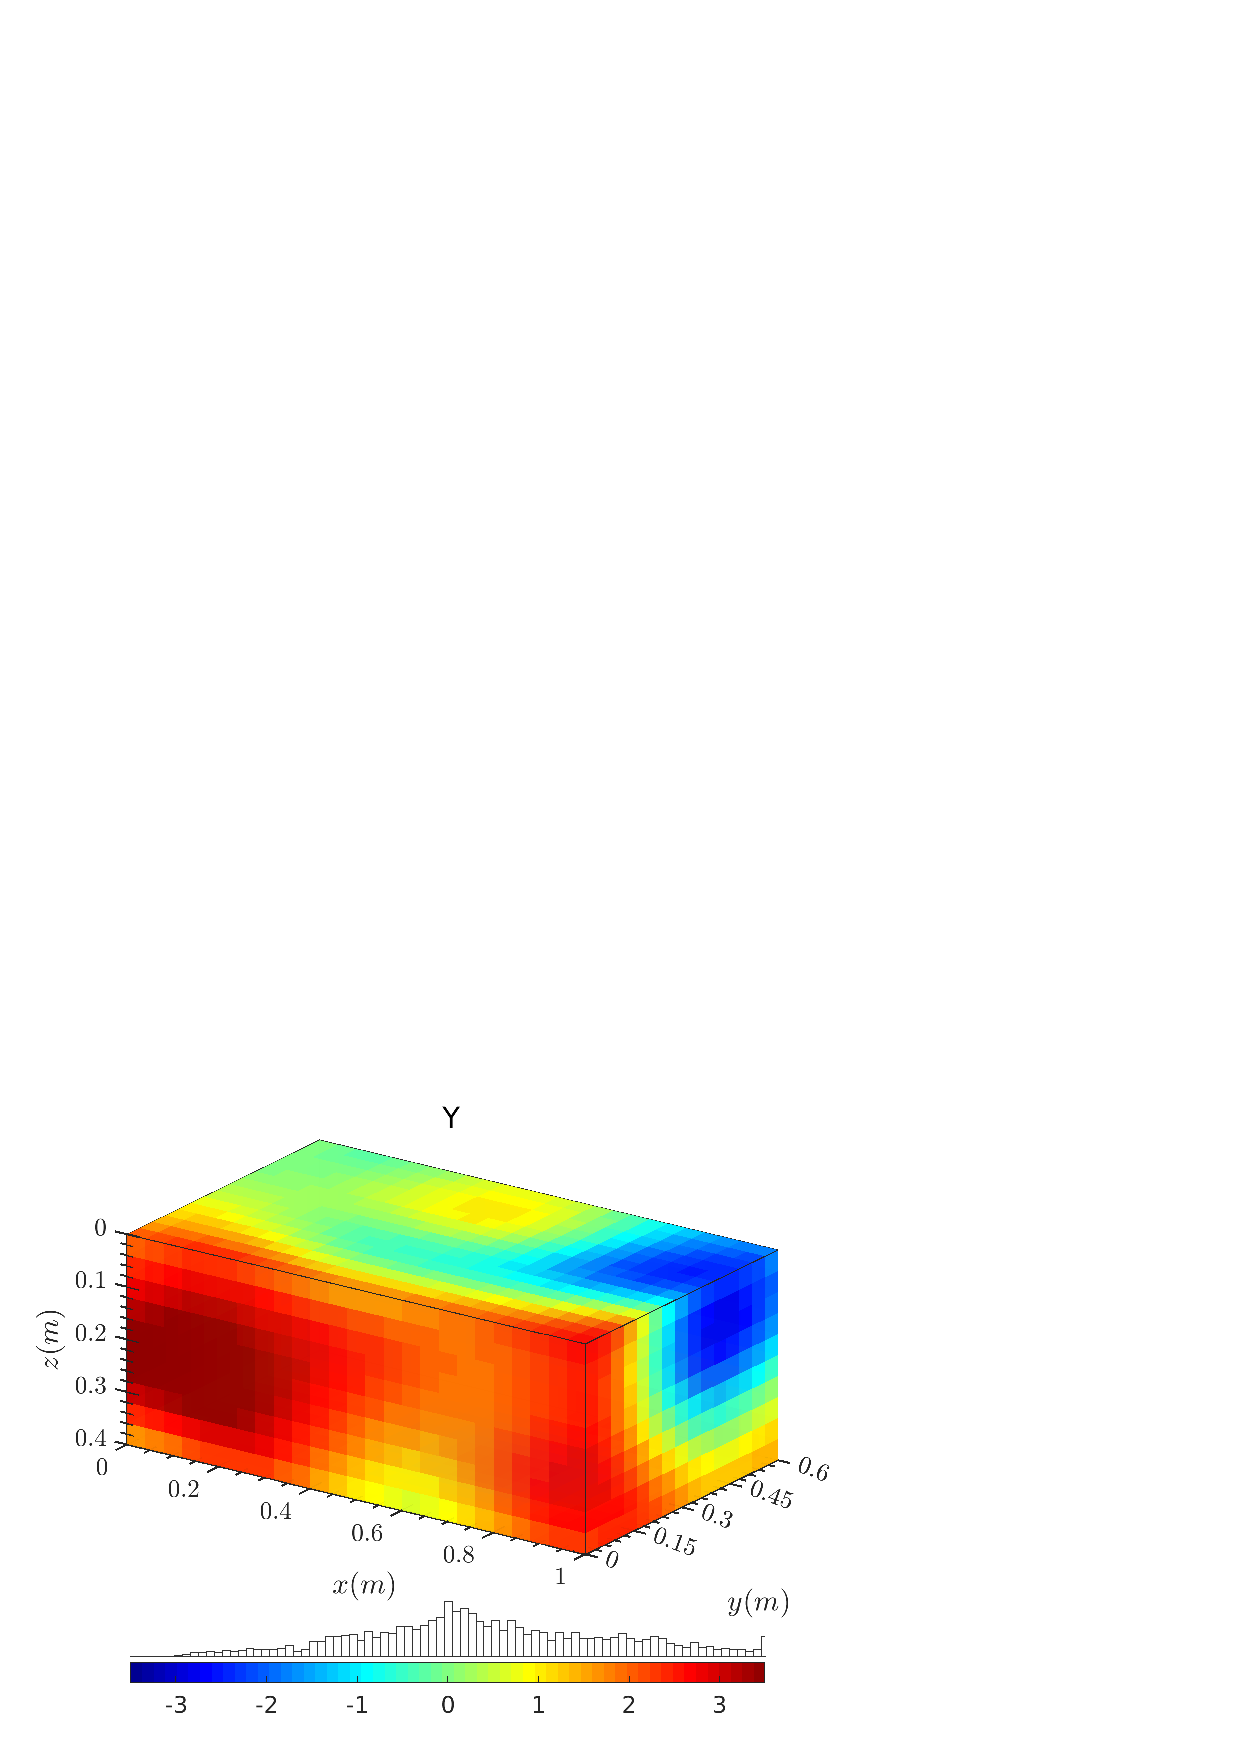
\includegraphics[scale=0.5]{./figuras/Y_sexpUNCOND_0.png}}
 \subfigure[]{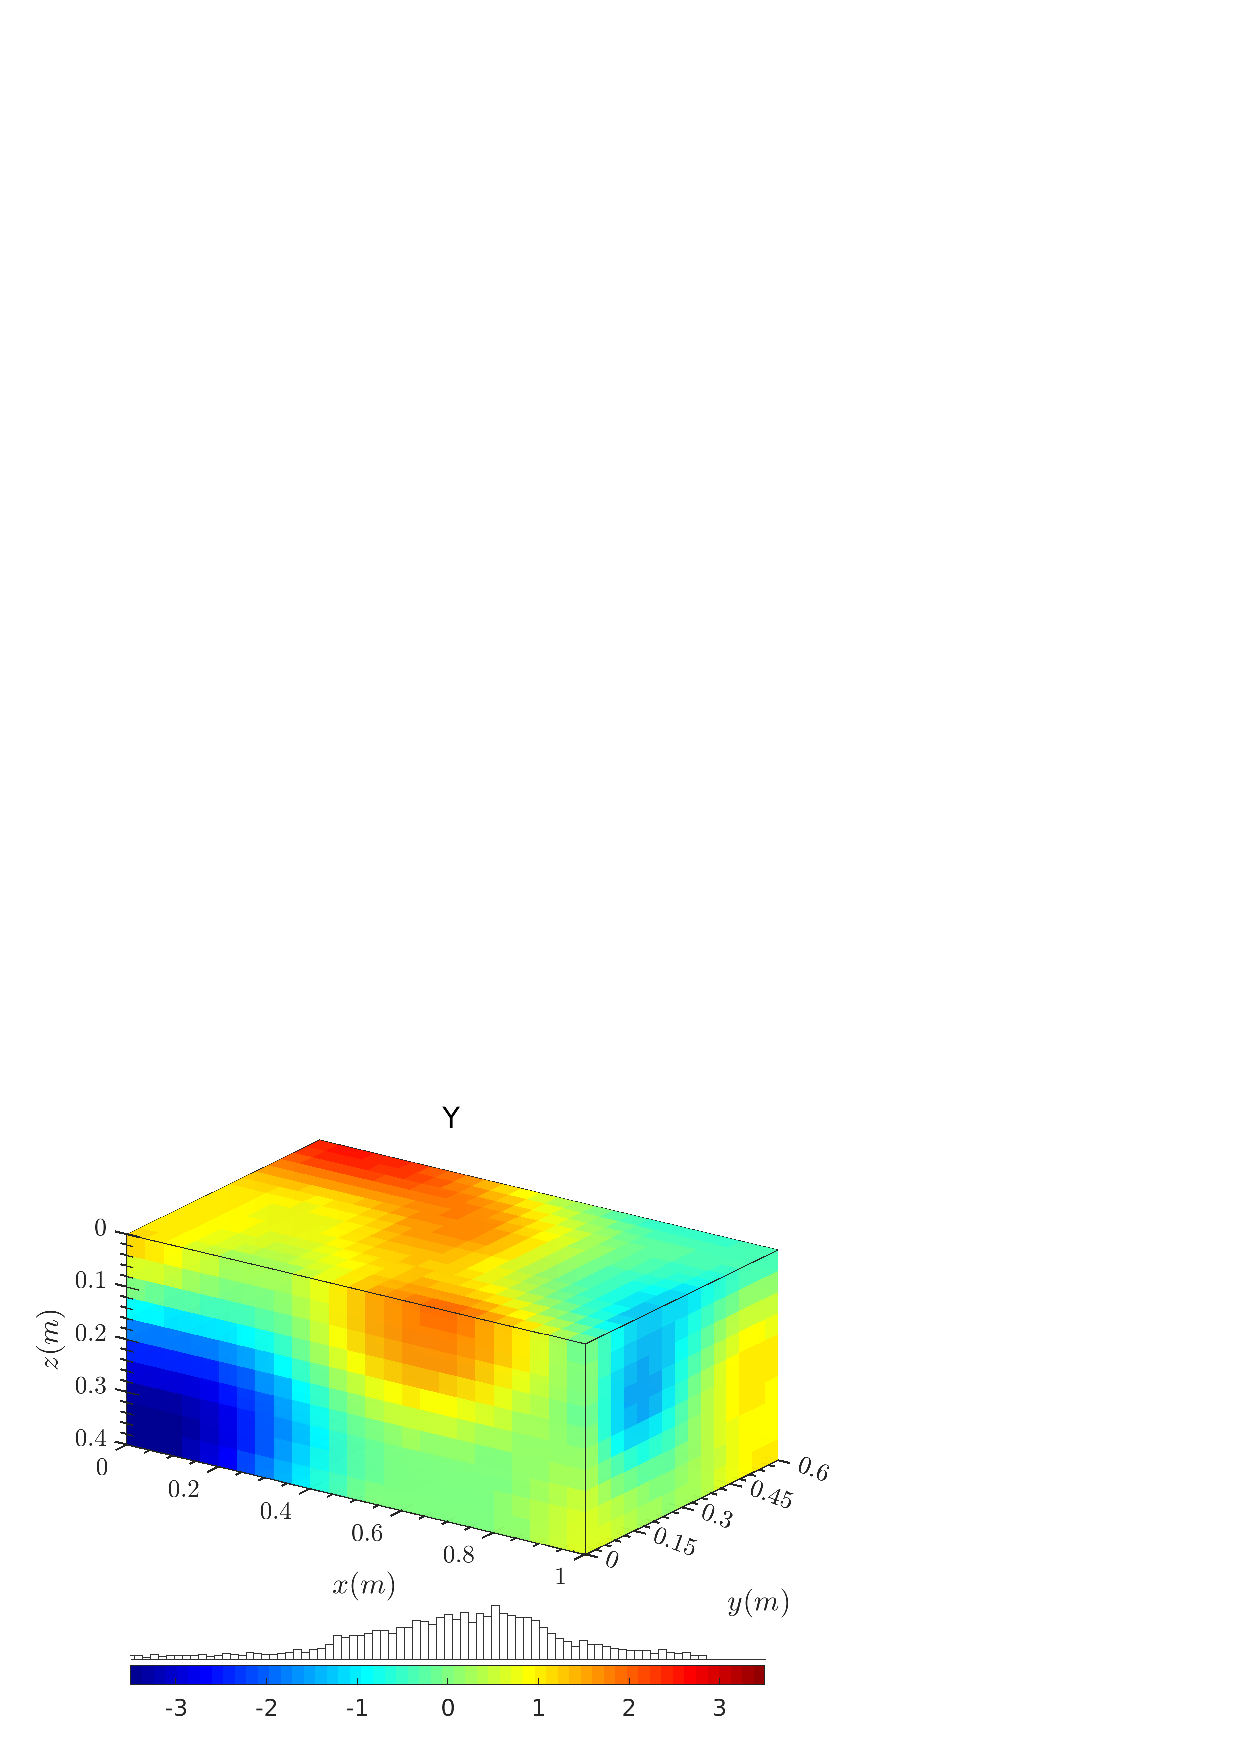
\includegraphics[scale=0.5]{./figuras/Y_sexpUNCOND_1.png}}
 \subfigure[]{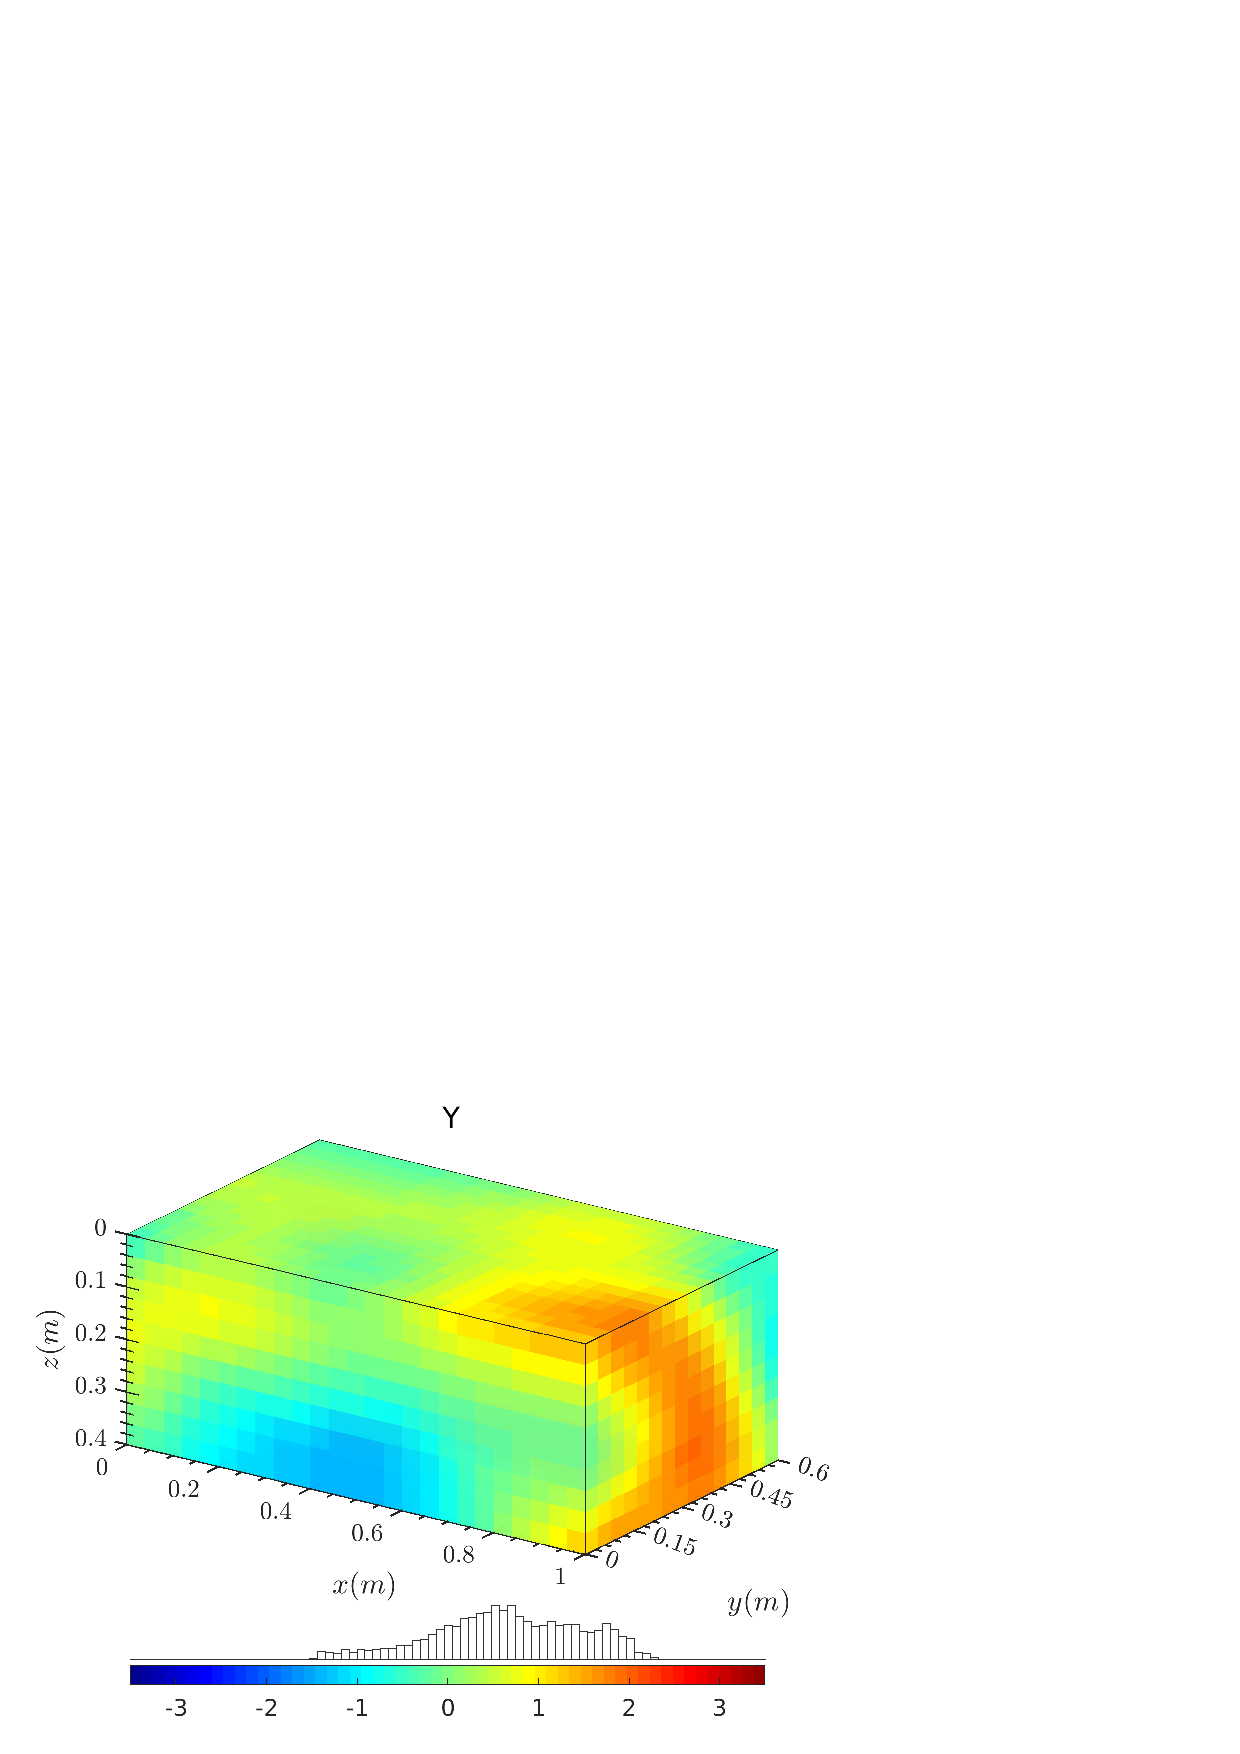
\includegraphics[scale=0.5]{./figuras/Y_sexpUNCOND_2.png}}
 \subfigure[]{\includegraphics[scale=0.5]{./figuras/Y_sexpUNCOND_3.png}}
 \caption{Realizations of random fields with squared exponential covariance (\eq{eq-squarecov}).}
 \label{fig-uncondFields}
\end{figure}


\fig{fig-uncondCov} shows the computed covariance function obtained with 2000 realizations. 
The models obtained (red line) by fitting the computed points are in excellent agreement with the theoretical model (\eq{eq-squarecov}).

\begin{figure}[H]
 \centering
 \subfigure[Direction $x$]{\includegraphics[scale = 0.325]{./figuras/e_gsexp_1x0_6x0_4_25x15x10_0-2x0-2x0-1_5000_Yx.png}}
 \subfigure[Direction $y$]{\includegraphics[scale = 0.325]{./figuras/e_gsexp_1x0_6x0_4_25x15x10_0-2x0-2x0-1_5000_Yy.png}}
 \subfigure[Direction $z$]{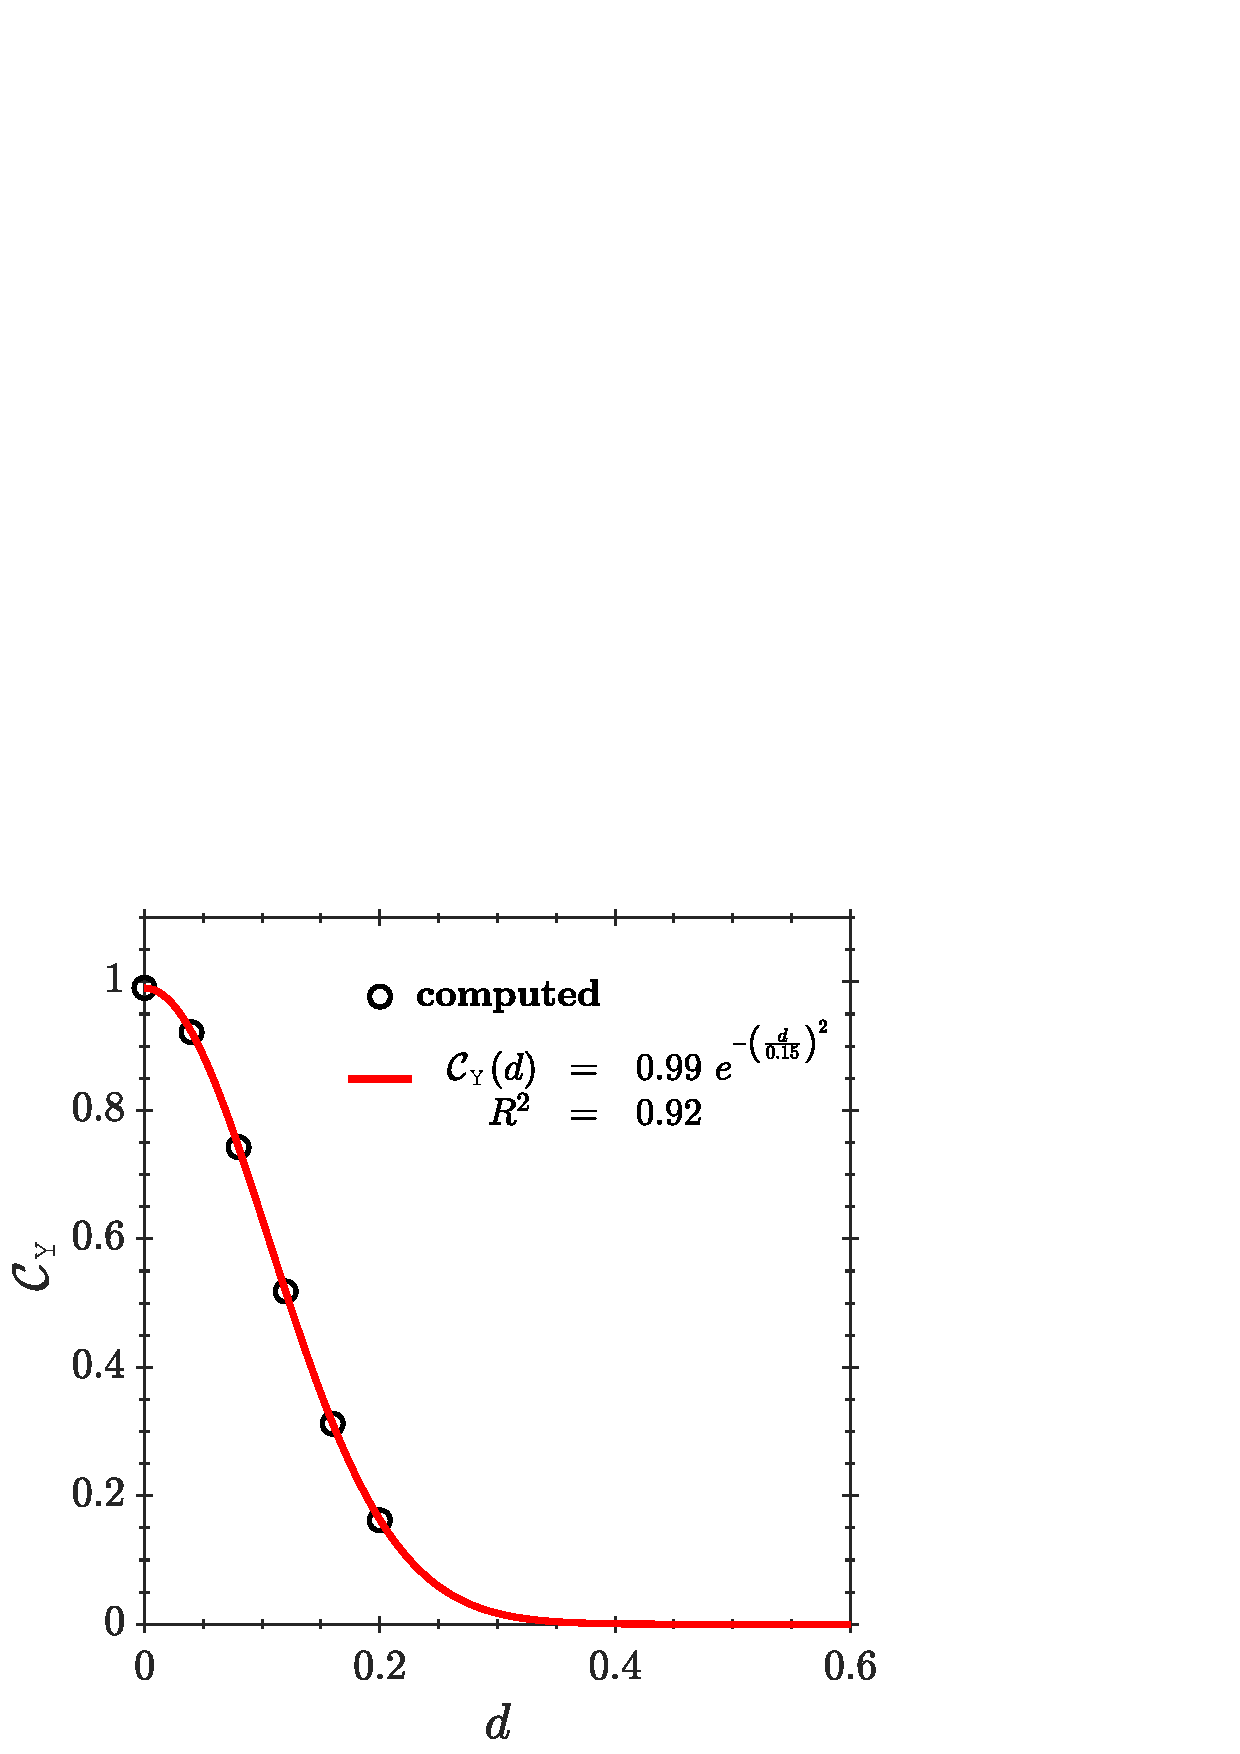
\includegraphics[scale = 0.325]{./figuras/e_gsexp_1x0_6x0_4_25x15x10_0-2x0-2x0-1_5000_Yz.png}}
 \caption{Covariance as function of the lag distance $d=\lVert \vx - \vy \rVert$, computed with an ensamble of 2000 unconditioned fields.}
 \label{fig-uncondCov}
\end{figure}

%%%%%%%%%%%%%%%%%%%%%%%%%%%%%%%%%%%%%%%%%%%%%%%%%%%%%%%%%%%%%%%%%%
\subsubsection{Conditioned}

In this section, an experiment similar to the previous one is conducted, however, the fields are conditioned at four points, as shown in the \tab{tab-cond}.

% \begin{table}[H]
%  \caption{Conditioned points}\label{tab-cond}
% \begin{center}
% \begin{tabular}{cccc}\hline\hline
% $x$ & $y$ & $z$ & $\Y\fx$\\ \hline
% 0.125 & 0.025 & 0.375 & 1.000\\
% 0.575 & 0.025 & 0.125 & 1.000\\
% 0.975 & 0.175 & 0.225 & -1.000\\
% 0.975 & 0.525 & 0.175 & -1.000\\ \hline\hline
% \end{tabular}
% \end{center}
% \end{table}

{%
\begin{table}[H]
 \caption{Conditioned points}\label{tab-cond}
\newcommand{\mc}[3]{\multicolumn{#1}{#2}{#3}}
\begin{center}
\begin{tabular}{cllc}
\hline\hline
\mc{3}{c}{{Point $\vx$}} & \\
$x$ & \mc{1}{c}{$y$} & \mc{1}{c}{$z$} & $\Y\fx$\\ \hline
0.125 & \mc{1}{c}{0.025} & \mc{1}{c}{0.375} & 1.000\\
0.575 & \mc{1}{c}{0.025} & \mc{1}{c}{0.125} & 1.000\\
0.975 & \mc{1}{c}{0.175} & \mc{1}{c}{0.225} & -1.000\\
0.975 & \mc{1}{c}{0.525} & \mc{1}{c}{0.175} & -1.000\\ \hline\hline
\end{tabular}
\end{center}
\end{table}
}%


In \fig{fig-condFields} two realizations of the fields are presented and the cubes show the conditioned points.

\begin{figure}[H]
 \centering
 \subfigure[]{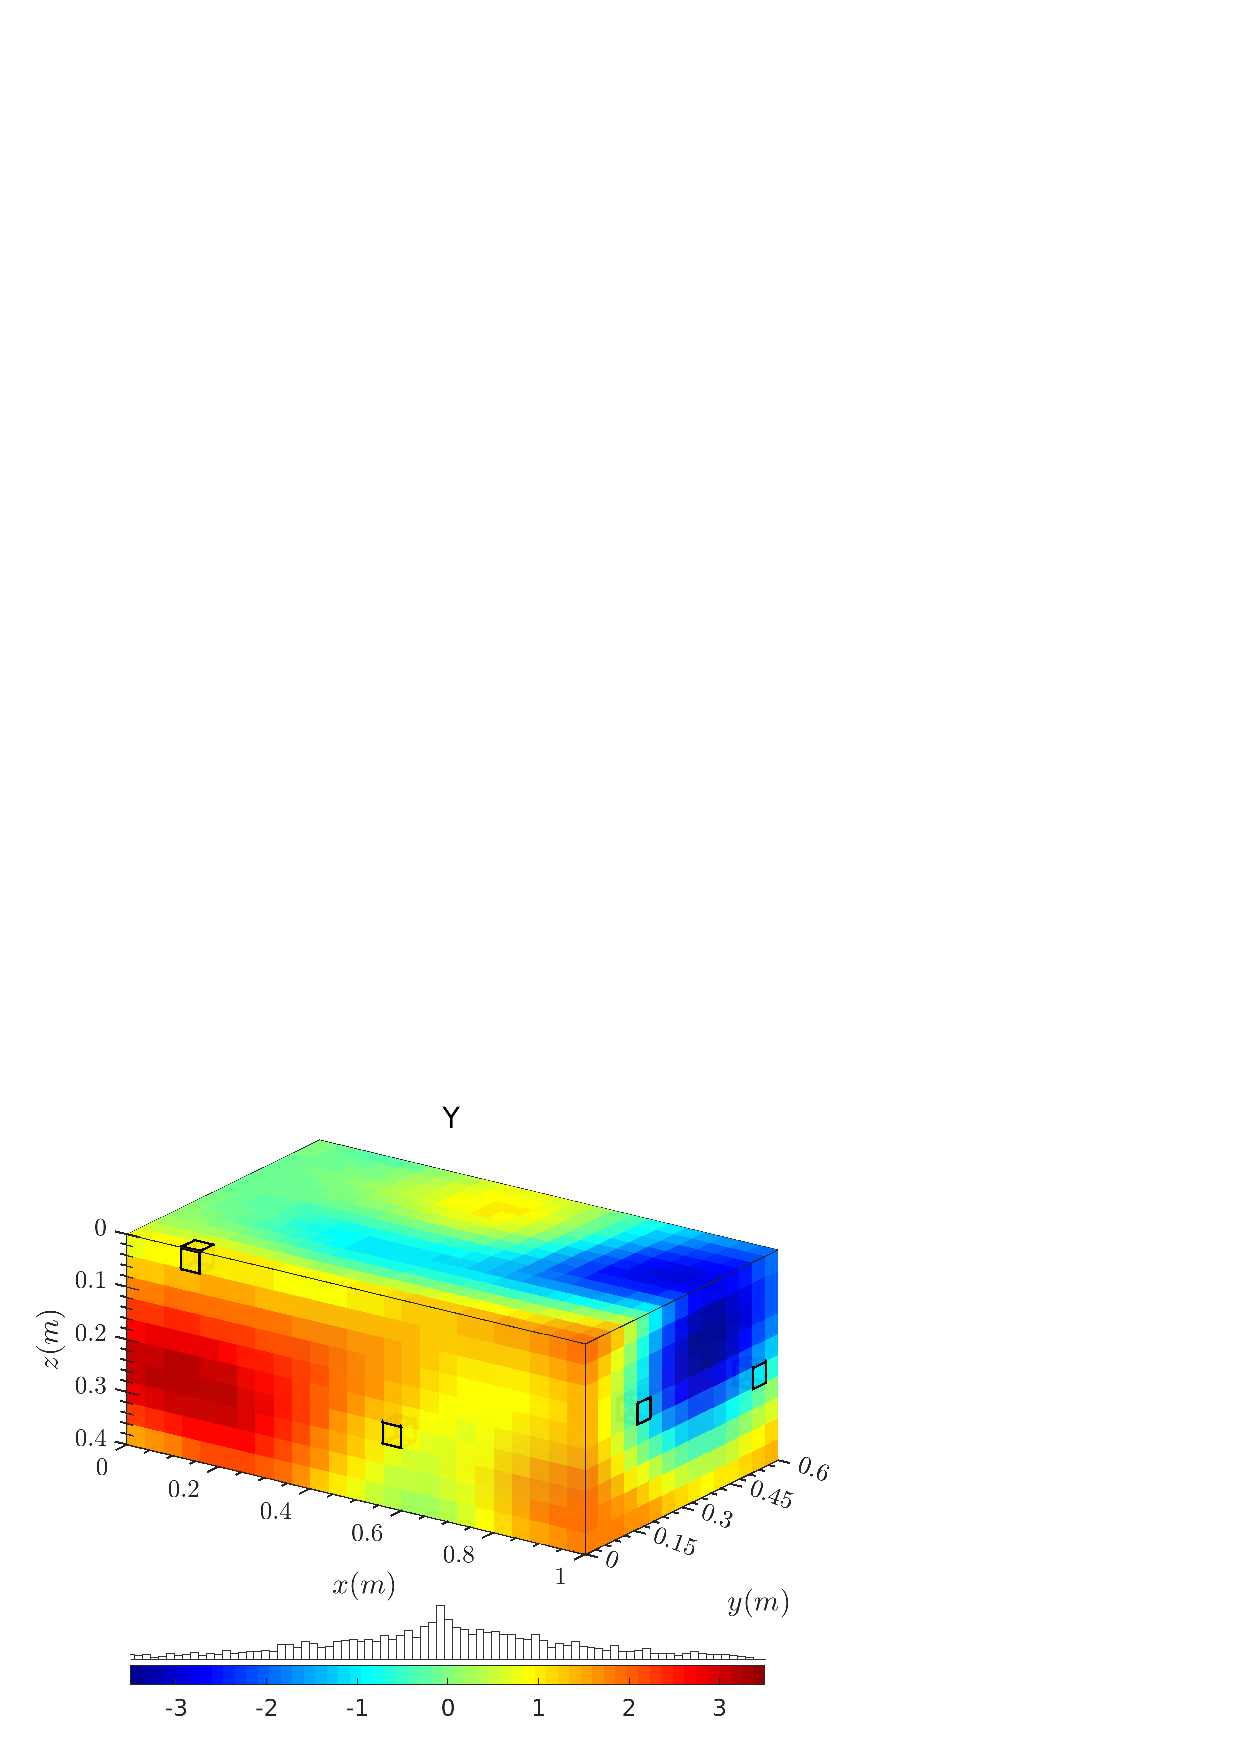
\includegraphics[scale=0.5]{./figuras/Y_sexpCOND_0.png}}
 \subfigure[]{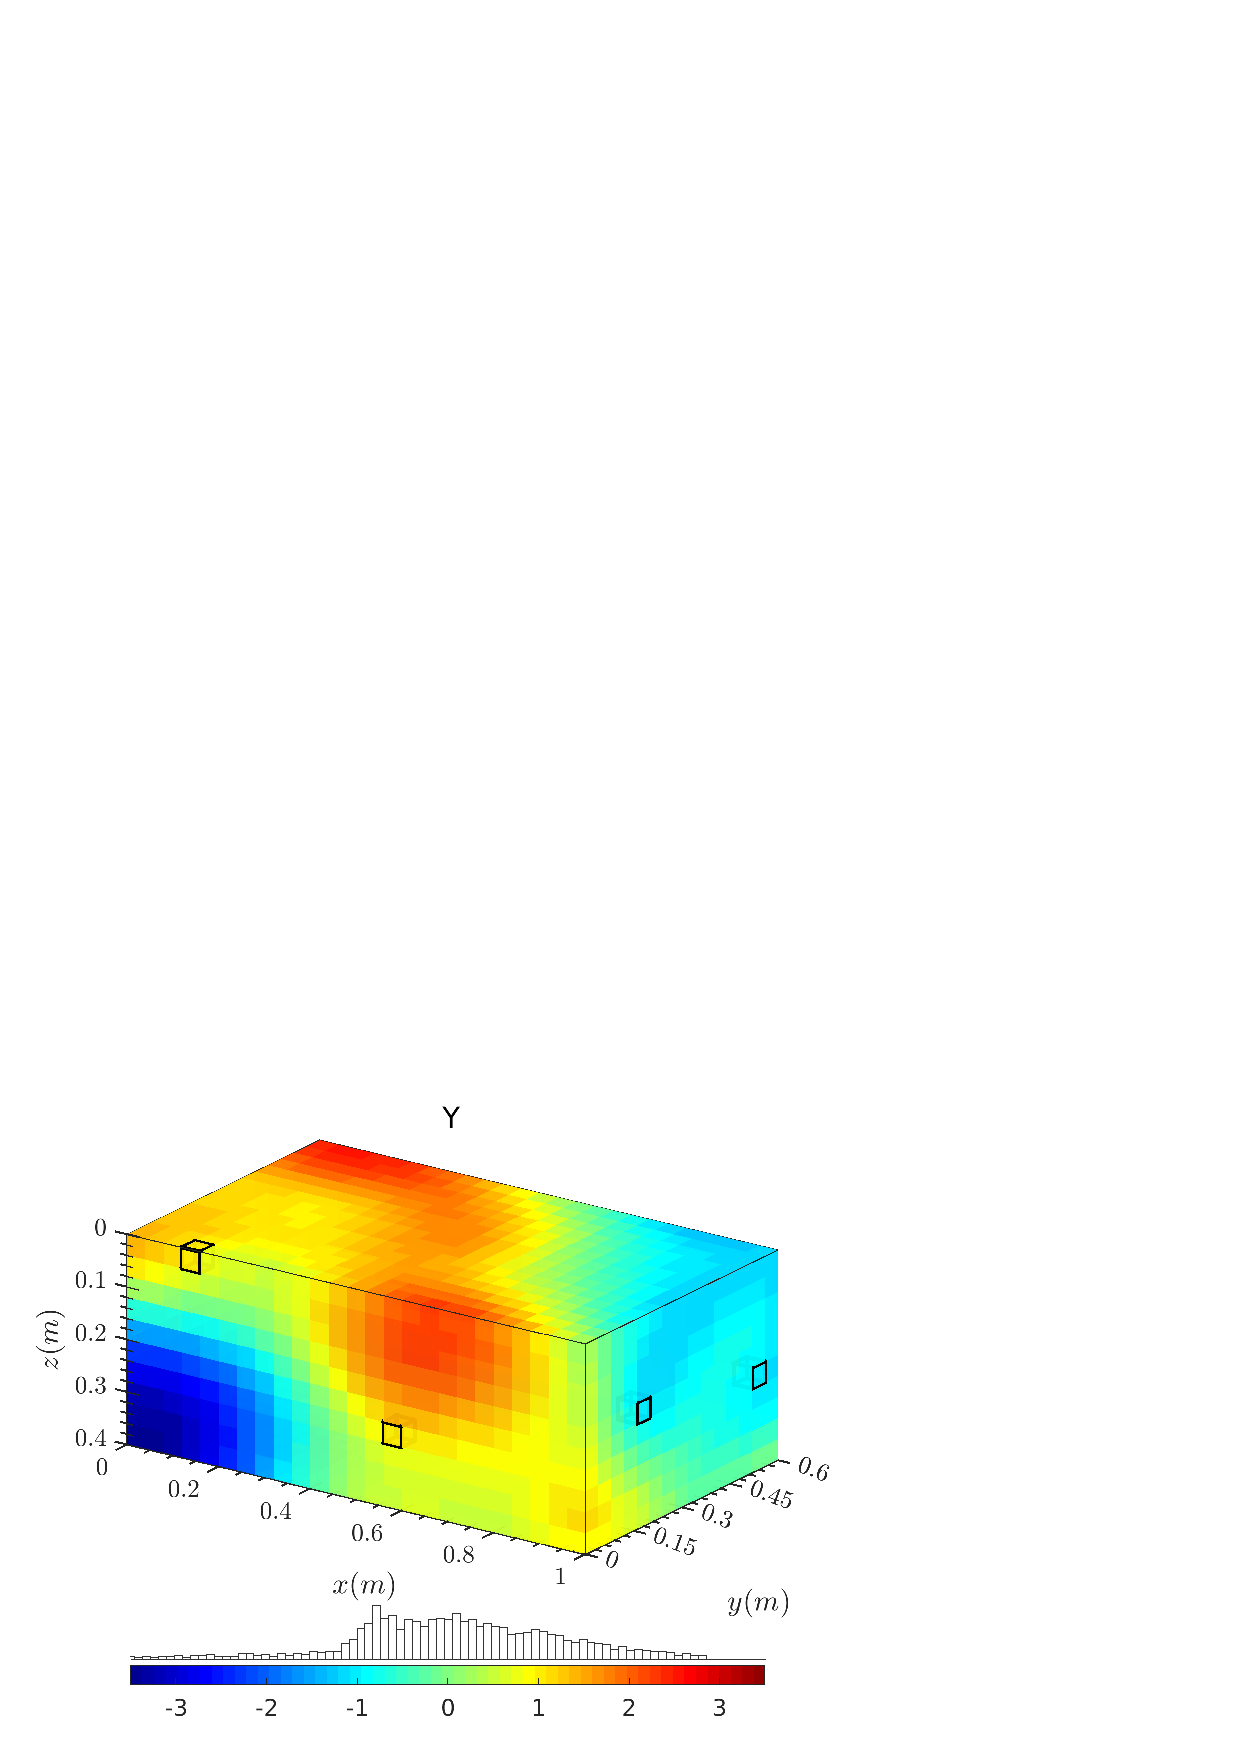
\includegraphics[scale=0.5]{./figuras/Y_sexpCOND_1.png}}
 \subfigure[]{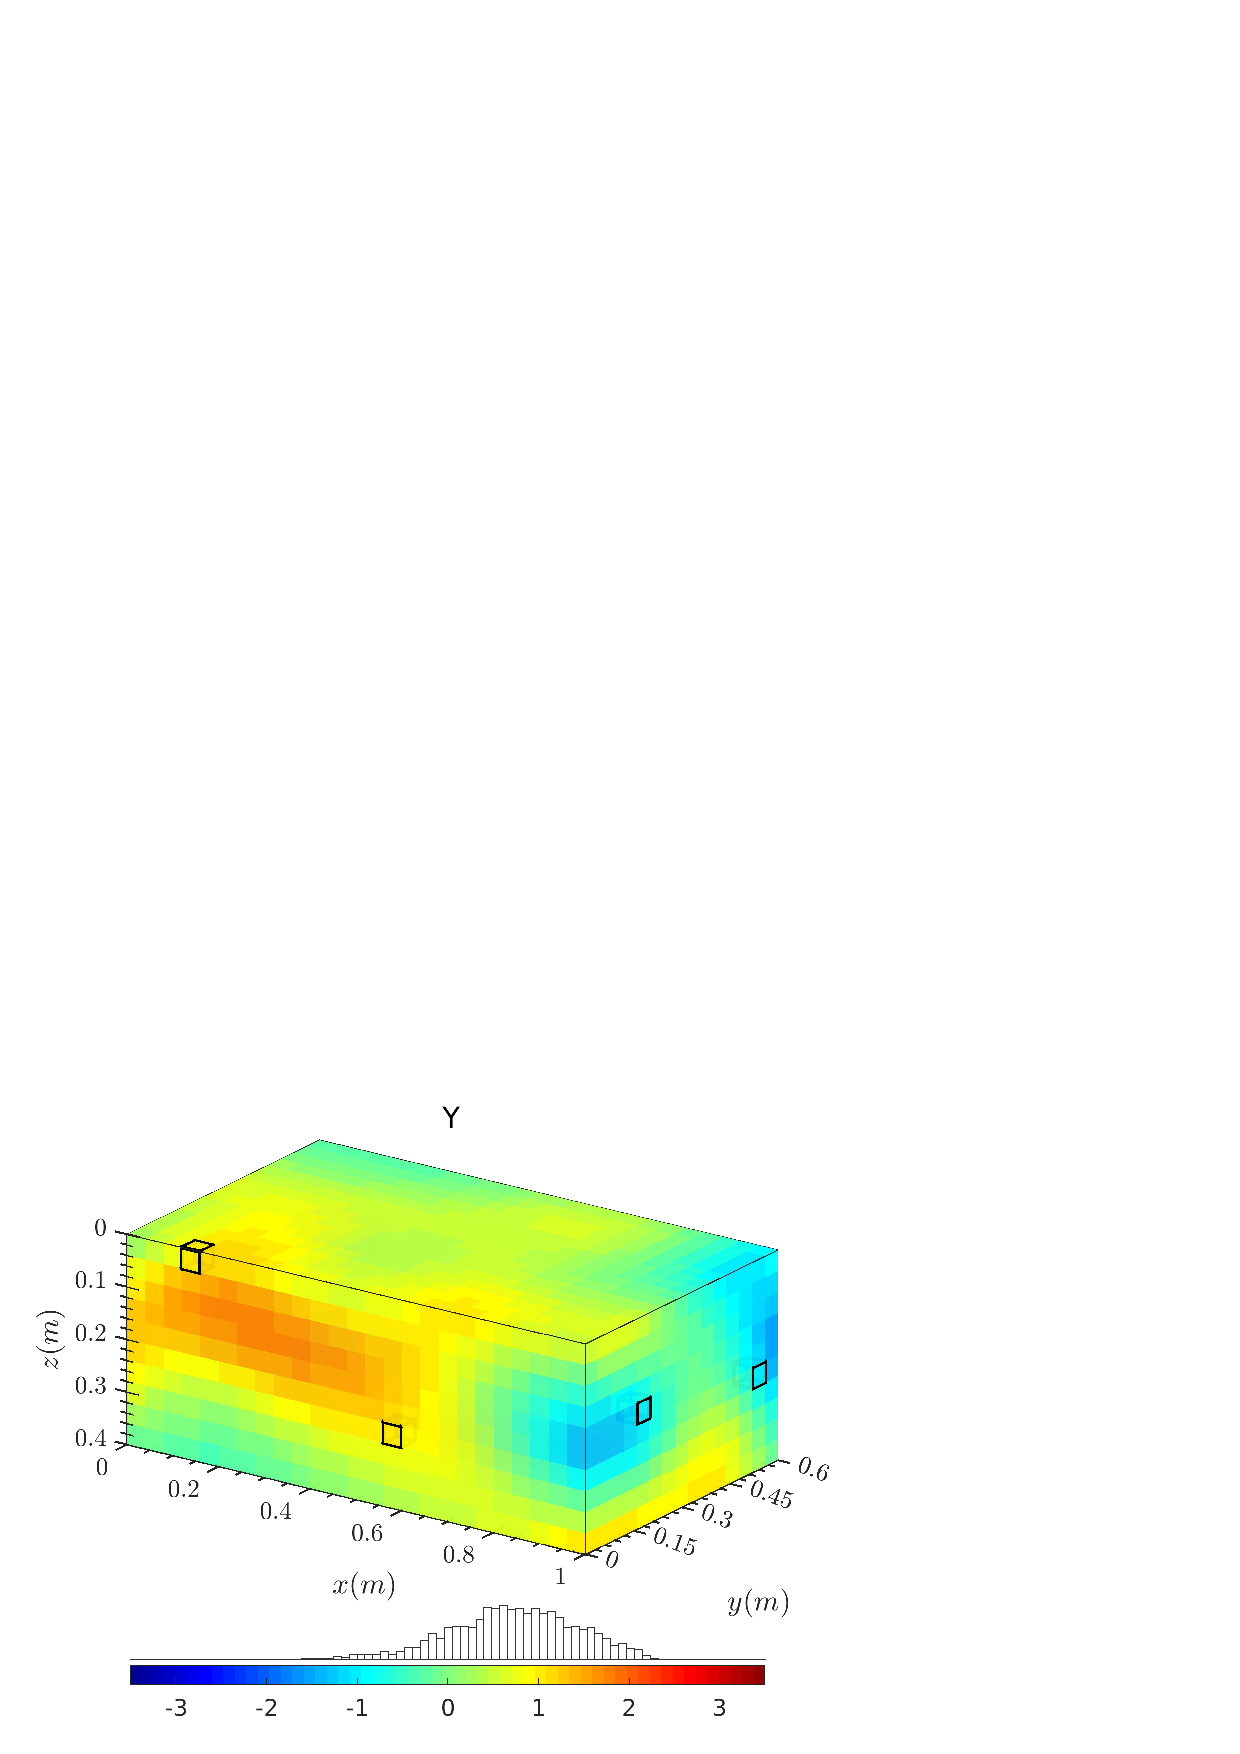
\includegraphics[scale=0.5]{./figuras/Y_sexpCOND_2.png}}
 \subfigure[]{\includegraphics[scale=0.5]{./figuras/Y_sexpCOND_3.png}}
 \caption{Realizations of random fields with squared exponential covariance (\eq{eq-squarecov}).}
 \label{fig-condFields}
\end{figure}

\fig{fig-uncondCov} shows the computed covariance function obtained with 2000 realizations. 
The models obtained (red line) by fitting the computed points are in excellent agreement with the theoretical model (\eq{eq-squarecov}).

\begin{figure}[H]
 \centering
 \subfigure[Direction $x$]{\includegraphics[scale = 0.325]{./figuras/e_gsexp_cond_1x0_6x0_4_25x15x10_0-2x0-2x0-1_5000_Yx.png}}
 \subfigure[Direction $y$]{\includegraphics[scale = 0.325]{./figuras/e_gsexp_cond_1x0_6x0_4_25x15x10_0-2x0-2x0-1_5000_Yy.png}}
 \subfigure[Direction $z$]{\includegraphics[scale = 0.325]{./figuras/e_gsexp_cond_1x0_6x0_4_25x15x10_0-2x0-2x0-1_5000_Yz.png}}
 \caption{Covariance as function of the lag distance $d=\lVert \vx - \vy \rVert$, computed with an ensamble of 2000 unconditioned fields.}
 \label{fig-uncondCov}
\end{figure}

%%%%%%%%%%%%%%%%%%%%%%%%%%%%%%%%%%%%%%%%%%%%%%%%%%%%%%%%%%%%%%%%%%
%%%%%%%%%%%%%%%%%%%%%%%%%%%%%%%%%%%%%%%%%%%%%%%%%%%%%%%%%%%%%%%%%%
\section{Synthetic experiment}
%%%%%%%%%%%%%%%%%%%%%%%%%%%%%%%%%%%%%%%%%%%%%%%%%%%%%%%%%%%%%%%%%%

We consider three-dimensional fields with dimensions: $36.0 \times 36.0 \times 50.0$ [$mm~\times~mm~\times~mm$] and mesh $36 \times 36 \times 50$.
Two kind of two-point covariance functions are considered:

\begin{itemize}
 \item Exponentially decaying covariance
 \begin{equation}
 \covv{\Y} = \vari{\Y}\exp\left(-\dfrac{\norma{x_1 - y_1}}{\cc_{1}}-\dfrac{\norma{x_2 - y_2}}{\cc_{2}}-\dfrac{\norma{x_3 - y_3}}{\cc_{3}}  \right),
 \label{eq-expcov}
\end{equation}

 \item Squared exponentially decaying covariance
\begin{equation}
 \covv{\Y} = \vari{\Y}\exp\left(-\dfrac{\norma{x_1 - y_1}^2}{\cc_{1}^{2}}-\dfrac{\norma{x_2 - y_2}^2}{\cc_{2}^{2}}-\dfrac{\norma{x_3 - y_3}^2}{\cc_{3}^{2}}  \right),
 \label{eq-squarecov}
\end{equation}
\end{itemize}

\noindent with $\vari{\Y}$ denoting the variance and $\cc_{i}>0,\ i=1,2,3$ the correlation length in each cartesian direction.
The correlation lengths used  in this study are: $\ell_{1}=\ell_{2}=\ell_{3}=3.0mm$.

Samples of the fields generated with \kl\ expansion are displayed in \figsto{fig-field_exp}{fig-field_sexp}

\begin{figure}[H]
 \centering
 \subfigure[Exponential]{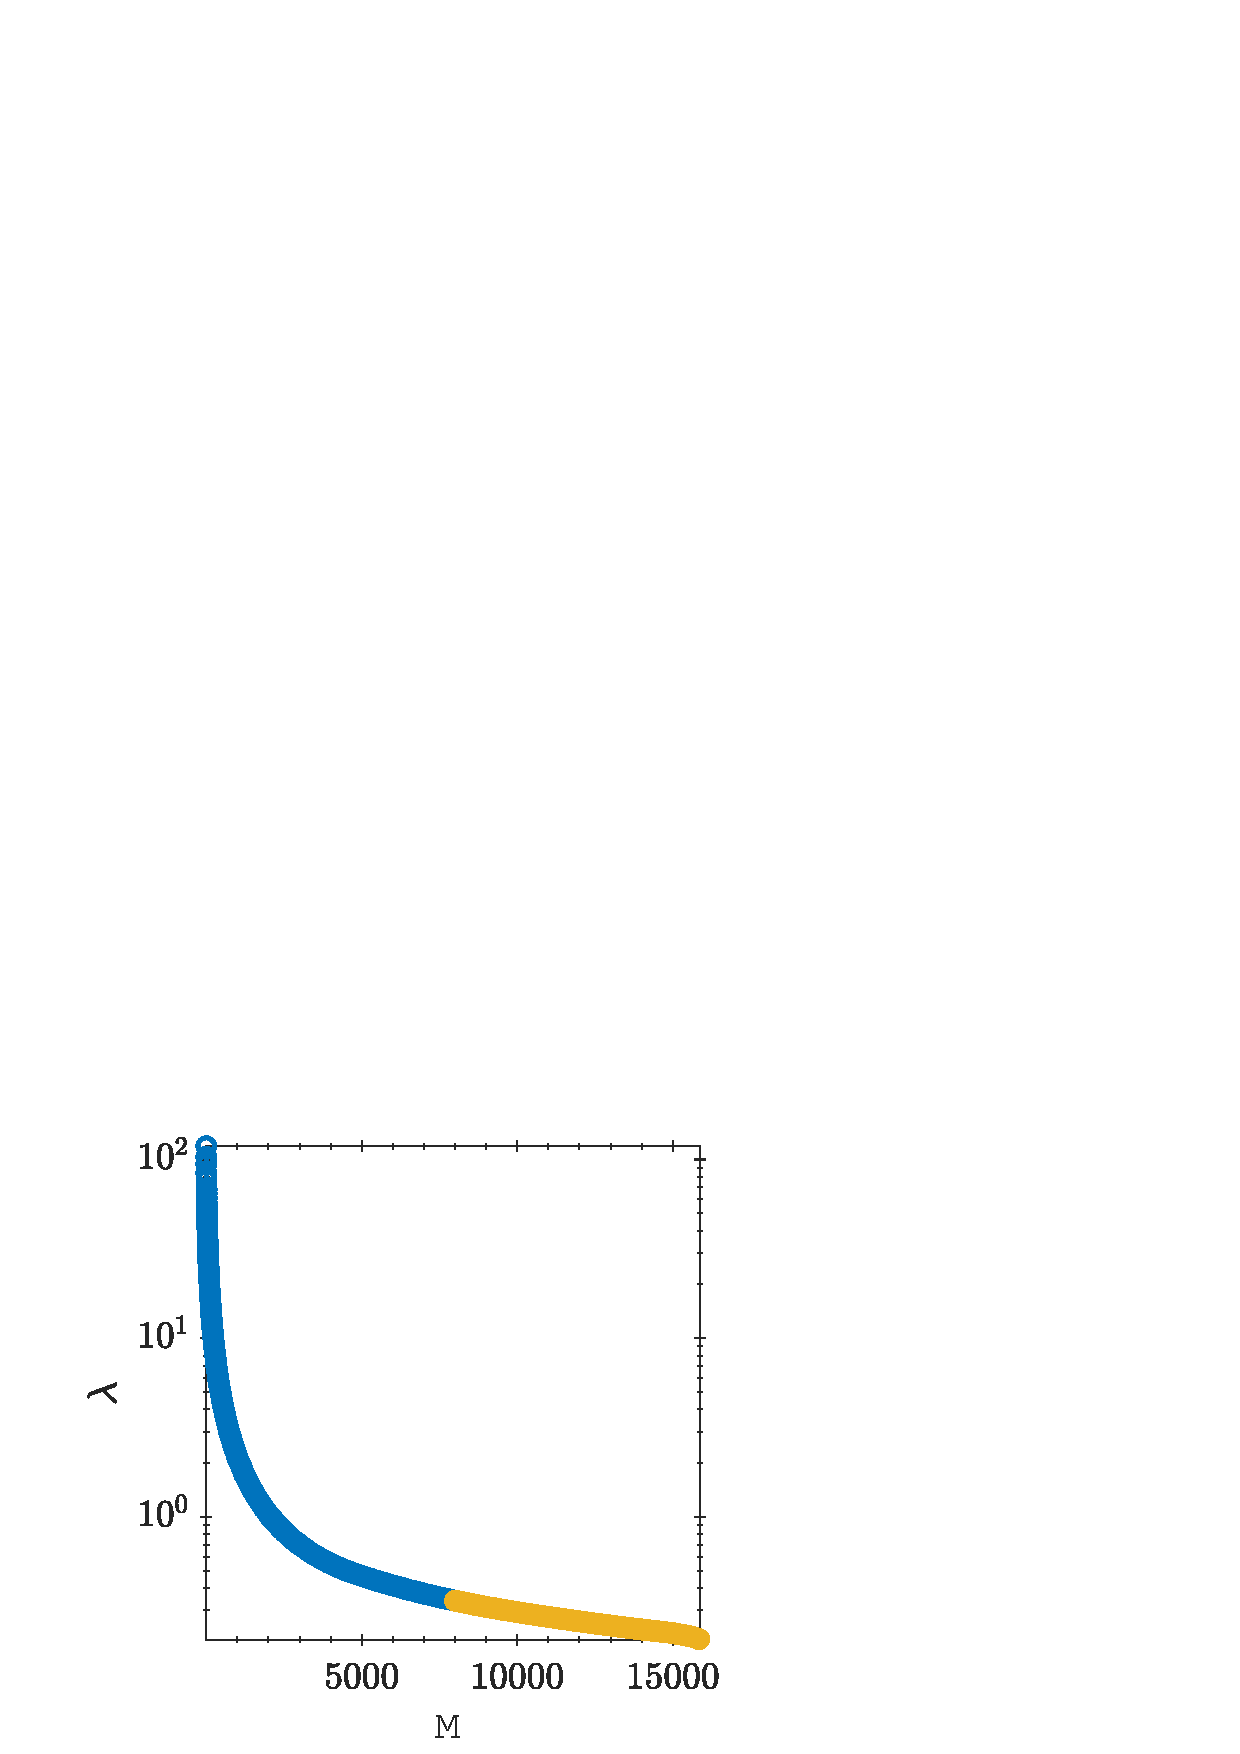
\includegraphics[scale=0.5]{./figuras/exp_autoval_36x36x50_3x3x3_8000.png}}
 \subfigure[Square exponential]{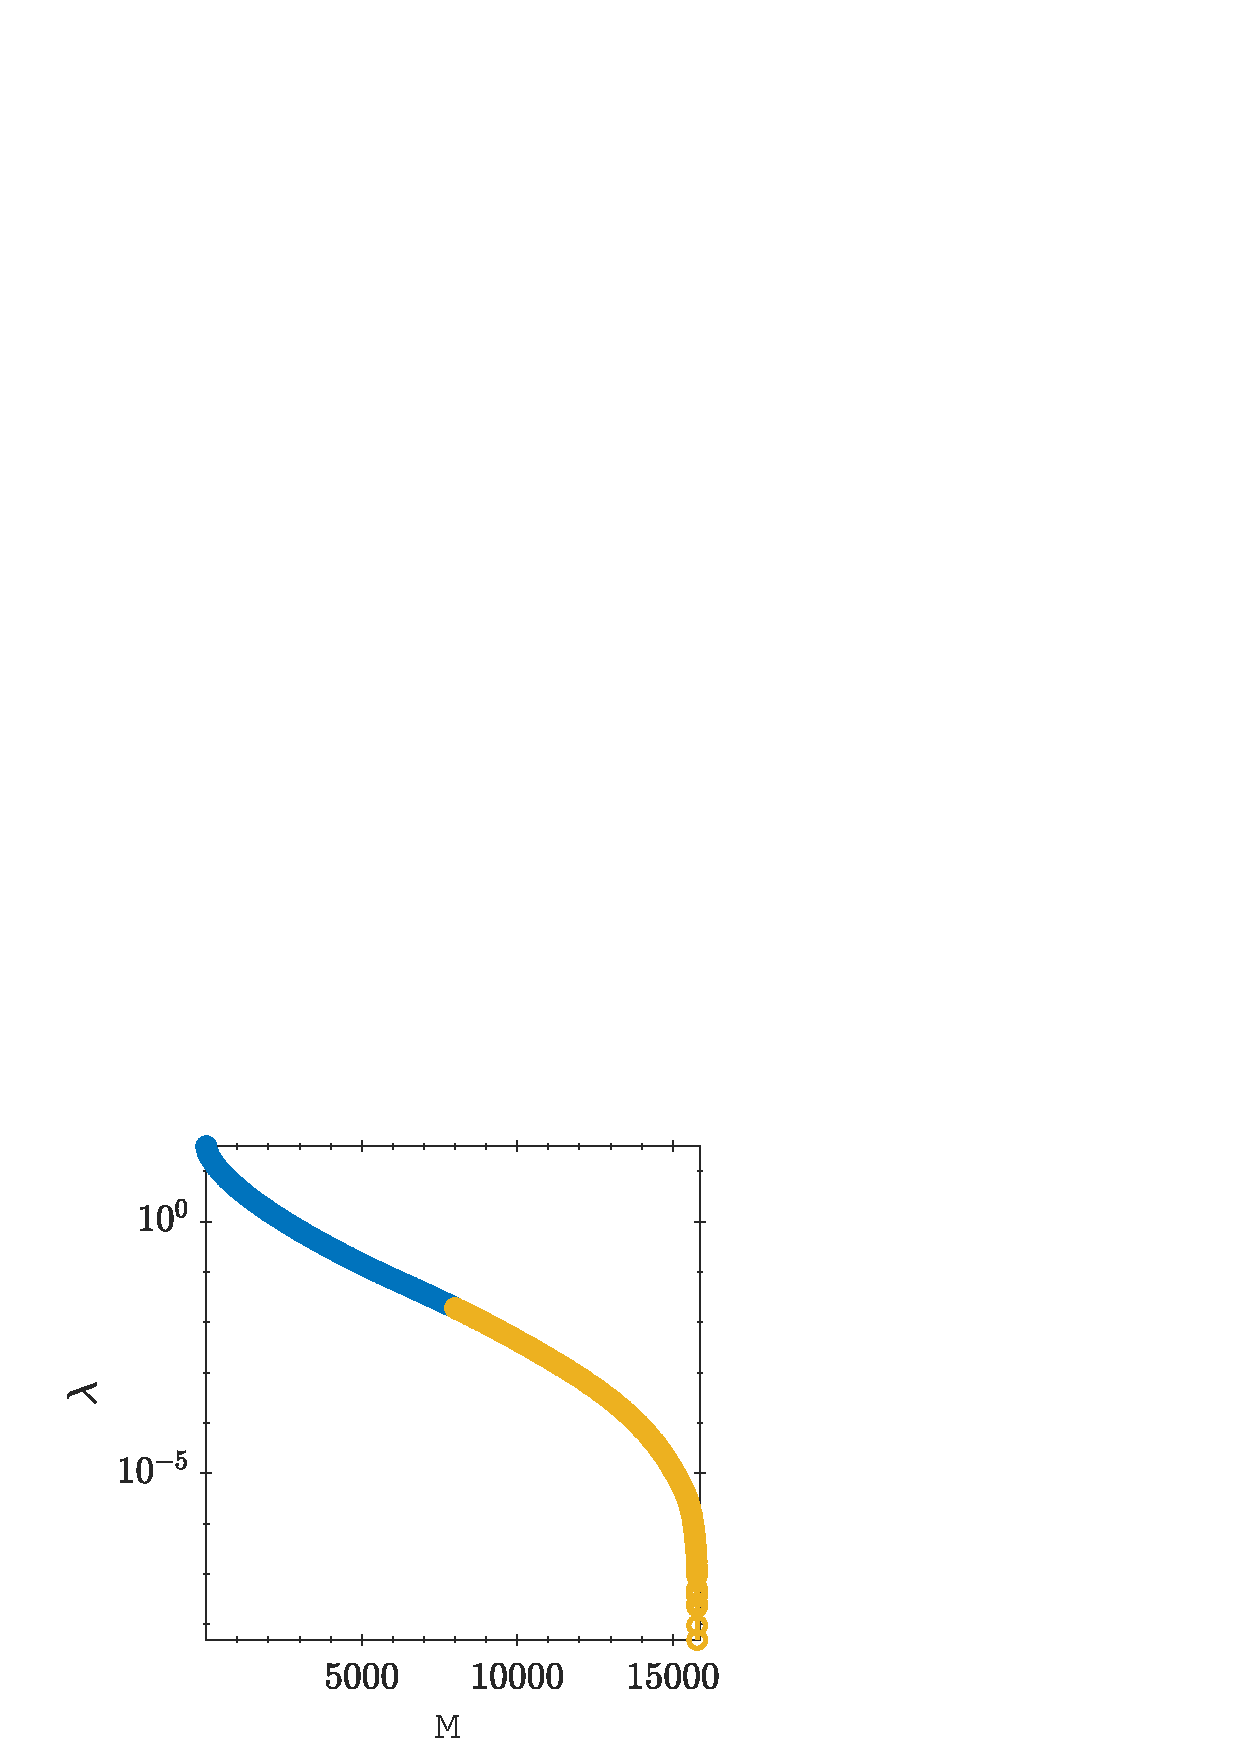
\includegraphics[scale=0.5]{./figuras/sexp_autoval_36x36x50_3x3x3_8000.png}}
 \caption{Eigenvalues of the covariance (\eq{kl}) as function of the number of terms in descending order.}
 \label{eigenval}
\end{figure}

%%%%%%%%%%%%%%%%%%%%%%%%%%%%%%%%%%%%%%%%%%%%%%%%%%%%%%%%%%%%%%%%%%
\begin{figure}[H]
 \centering
 \subfigure[]{\includegraphics[scale=0.525]{./figuras/Y_TUBexpUNCOND_0.png}}
 \subfigure[]{\includegraphics[scale=0.525]{./figuras/Y_TUBexpUNCOND_1.png}}
 \subfigure[]{\includegraphics[scale=0.525]{./figuras/Y_TUBexpUNCOND_2.png}}
 \subfigure[]{\includegraphics[scale=0.525]{./figuras/Y_TUBexpUNCOND_3.png}}
 \caption{Samples of random fields with exponentially decay covariance.}
 \label{fig-field_exp}
\end{figure}

%%%%%%%%%%%%%%%%%%%%%%%%%%%%%%%%%%%%%%%%%%%%%%%%%%%%%%%%%%%%%%%%%%
\begin{figure}[H]
 \centering
 \subfigure[]{\includegraphics[scale=0.525]{./figuras/Y_TUBsexpCOND_0.png}}
 \subfigure[]{\includegraphics[scale=0.525]{./figuras/Y_TUBsexpCOND_1.png}}
 \subfigure[]{\includegraphics[scale=0.525]{./figuras/Y_TUBsexpCOND_2.png}}
 \subfigure[]{\includegraphics[scale=0.525]{./figuras/Y_TUBsexpCOND_3.png}}
 \caption{Samples of random fields with exponentially decay covariance.}
 \label{fig-field_sexp}
\end{figure}

%%%%%%%%%%%%%%%%%%%%%%%%%%%%%%%%%%%%%%%%%%%%%%%%%%%%%%%%%%%%%%%%%%
%%%%%%%%%%%%%%%%%%%%%%%%%%%%%%%%%%%%%%%%%%%%%%%%%%%%%%%%%%%%%%%%%%
%%%%%%%%%%%%%%%%%%%%%%%%%%%%%%%%%%%%%%%%%%%%%%%%%%%%%%%%%%%%%%%%%%
%%%%%%%%%%%%%%%%%%%%%%%%%%%%%%%%%%%%%%%%%%%%%%%%%%%%%%%%%%%%%%%%%%
%%%%%%%%%%%%%%%%%%%%%%%%%%%%%%%%%%%%%%%%%%%%%%%%%%%%%%%%%%%%%%%%%%
%%%%%%%%%%%%%%%%%%%%%%%%%%%%%%%%%%%%%%%%%%%%%%%%%%%%%%%%%%%%%%%%%%


% \begin{figure}[H]
%  \centering
%  \subfigure[Direction $x$]{\includegraphics[scale=0.325]{./figuras/e_gexp_40x40x40_20x20x20_10x8x6_2000_Yx.png}}
%  \subfigure[Direction $y$]{\includegraphics[scale=0.325]{./figuras/e_gexp_40x40x40_20x20x20_10x8x6_2000_Yy.png}}
%  \subfigure[Direction $z$]{\includegraphics[scale=0.325]{./figuras/e_gexp_40x40x40_20x20x20_10x8x6_2000_Yz.png}}
%  \subfigure[Direction $x$]{\includegraphics[scale=0.325]{./figuras/eIn_gexp_40x40x40_20x20x20_10x8x6_2000_Yx.png}}
%  \subfigure[Direction $y$]{\includegraphics[scale=0.325]{./figuras/eIn_gexp_40x40x40_20x20x20_10x8x6_2000_Yy.png}}
%  \subfigure[Direction $z$]{\includegraphics[scale=0.325]{./figuras/eIn_gexp_40x40x40_20x20x20_10x8x6_2000_Yz.png}}
%  \subfigure[Direction $x$]{\includegraphics[scale=0.325]{./figuras/eM_gexp_40x40x40_20x20x20_10x8x6_2000_Yx.png}}
%  \subfigure[Direction $y$]{\includegraphics[scale=0.325]{./figuras/eM_gexp_40x40x40_20x20x20_10x8x6_2000_Yy.png}}
%  \subfigure[Direction $z$]{\includegraphics[scale=0.325]{./figuras/eM_gexp_40x40x40_20x20x20_10x8x6_2000_Yz.png}}
%  \caption{Computed covariance as function of the lag distance $r=\lVert \vx - \vy \rVert$.}
%  \label{figcovexp}
% \end{figure}
% 
% \begin{figure}[H]
%  \centering
%  \subfigure[Direction $x$]{\includegraphics[scale=0.325]{./figuras/e_gsexp_40x40x40_20x20x20_10x8x6_2000_Yx.png}}
%  \subfigure[Direction $y$]{\includegraphics[scale=0.325]{./figuras/e_gsexp_40x40x40_20x20x20_10x8x6_2000_Yy.png}}
%  \subfigure[Direction $z$]{\includegraphics[scale=0.325]{./figuras/e_gsexp_40x40x40_20x20x20_10x8x6_2000_Yz.png}}
%  \subfigure[Direction $x$]{\includegraphics[scale=0.325]{./figuras/eIn_gsexp_40x40x40_20x20x20_10x8x6_2000_Yx.png}}
%  \subfigure[Direction $y$]{\includegraphics[scale=0.325]{./figuras/eIn_gsexp_40x40x40_20x20x20_10x8x6_2000_Yy.png}}
%  \subfigure[Direction $z$]{\includegraphics[scale=0.325]{./figuras/eIn_gsexp_40x40x40_20x20x20_10x8x6_2000_Yz.png}}
%  \caption{Computed covariance as function of the lag distance $r=\lVert \vx - \vy \rVert$.}
%  \label{figcovexpf}
% \end{figure}
% 
% 
% \begin{figure}[H]
%  \centering
%  \subfigure[]{\includegraphics[scale=0.3]{./figuras/fields3D_cond_0001.png}}
%  \subfigure[]{\includegraphics[scale=0.3]{./figuras/fields3D_cond_0002.png}}\\
%  \subfigure[]{\includegraphics[scale=0.3]{./figuras/fields3D_cond_0003.png}}
%  \subfigure[]{\includegraphics[scale=0.3]{./figuras/fields3D_cond_0000.png}}
% \end{figure}




%%%%%%%%%%%%%%%%%%%%%%%%%%%%%%%%%%%%%%%%%%%%%%%%%%%%%%%%%%%%%%%%%%%%%%%%%%%
%\addcontentsline{toc}{chapter}{Bibliografia}
\bibliography{/prj/prjmurad/mrborges/Dropbox/latex/refbib/REFERENCIAS}
\bibliographystyle{/prj/prjmurad/mrborges/Dropbox/latex/refbib/plainnat}
%%%%%%%%%%%%%%%%%%%%%%%%%%%%%%%%%%%%%%%%%%%%%%%%%%%%%%%%%%%%%%%%%%%%%%%%%%%
%\clearpage
%\addcontentsline{toc}{chapter}{Índice}
%\printindex
%%%%%%%%%%%%%%%%%%%%%%%%%%%%%%%%%%%%%%%%%%%%%%%%%%%%%%%%%%%%%%%%%%%%%%%%%%%
\end{document}
